\todo{1. (30 min) Rewrite this intro}
In the rest of the chapter we develop an algorithm for generating failure descriptions and test it on the autonomous driving scenarios. Failures are described using signal temporal logic (STL) expressions. In the first section we give the necessary background for compactly representing STL using a context-free grammar, sampling STL expressions, and optimizing them using genetic programming. We then describe our approach for generating failure descriptions, which requires the ability to sample time series that satisfy a given STL expression. Our sampling procedure involves sampling a random set of linear constraints that, when imposed on a time series, ensures the satisfaction of the desired expression. Lastly, we demonstrate that the interpretable safety validation algorithm can find interpretable failure descriptions and produce a diverse set of failure examples. 

Lastly, we discuss techniques for modeling timeseries data that satisfy linear constraints including independent samples and series distributed according to a Gaussian process. 

\section{Background}

\todo{
2 - 30 min \\
- Describe the upside of scenario-based testing (i.e. that each scenario involves a semantically similar situation in the environment even if some of the variables change.  and explain that black box testing, in general does not have this feature \\
- Previous work -> Ritchie's work, as well as the airline setting?
- Create an example where one trajectory is a failure and one is not
}
% Introduce the problem (motivation)
One of the drawbacks to black-box safety validation techniques approaches is that they produce high-dimensional failure examples with no additional context about what it was about that trajectory that lead to a failures. 

% The approach we propose
Our approach seeks to find a \emph{failure description} $\varphi$ such that any disturbance trajectory that satisfies the description will cause the SUT to fail. For falsification we want to find any such $\varphi$ where
\begin{equation}
    \vec{x} \in \varphi \implies f(\vec{x}) \not \in \psi \text{.}
\end{equation}
For most likely failure analysis we want to find the $\varphi$ that produces failures with high likelihood
\begin{equation}
\max_\varphi \quad \mathbb{E}_{\vec{x} \sim p(\vec{x} \mid \vec{x} \in \varphi)}[p(\vec{x})] \quad\textrm{s.t.}\quad \vec{x} \in E
\end{equation}
where $p(\vec{x} \mid \vec{x} \in \varphi)$ is the probability density of disturbance trajectories that satisfy the description. 

\todo{2.5 - 10 min, Explain the broad approach that we have}

% Why is a fialure description a good thing?
A failure description $\varphi$ contains more information than a single failure example. For example, 
\todo{ 3 - 30 min \\
- A failure description can produce failure examples by sampling from $p(\vec{x} \mid \vec{x} \in \varphi)$.
- A failure example identifies the features of a disturbance trajectory that are sufficient to cause a failure (similar to a unit test). 
- Given a failure description we can perform a sensitivity analysis to find the failure boundary under certain scenarios. 
}



\section{STL Expression Optimization}
This section provides the necessary technical background to understand our approach for STL expression optimization. We first introduce context free grammars as a way to compactly represent signal temporal logic and describe how to sample valid STL expressions. We then describe genetic programming, a technique used to optimize tree-like structures such as STL expressions. Lastly, we introduce the failure description cost function that is used to find optimal failure descriptions.

\subsection{Context-Free Grammars}
\begin{figure}
    \centering
    \begin{forest}{for tree={ minimum size=1cm,}}
        [$\square$ 
            [$t_1$] 
            [$t_2$] 
            [$>$ 
                [$x$]
                [$0$]
            ]
        ]
    \end{forest}
    \caption{Expression tree for $\square_{[t_1, t_2]} x > 0$.}
    \label{fig:stl_tree}
\end{figure}

% Describing expressions as trees and grammar as a set of constraints
Logical expressions can be represented by a tree of symbols and operators. For example, the STL expression
\begin{equation}
    \square_{[t_1, t_2]} x > 0 \label{eq:example_stl_expression}
\end{equation}
can be represented by the tree shown in \cref{fig:stl_tree}. The semantics of a formal language specify a set of constraints on space of possible expression trees. These constraints can be compactly represented using a context-free grammar, which is a collection of production rules of the form
\begin{equation}
\mathbb{T} \mapsto \alpha,
\end{equation}
where $\mathbb{T}$ is a type and $\alpha$ is an expression that consists of types and symbols. A terminal production rule is one where $\alpha$ consists only of symbols. 

For example, the context-free grammar for a simplified version of STL for a single disturbance variable $x$ is given by
\begin{equation}
\label{eq:stl_grammar}
\begin{split}
    \mathbb{B} &\mapsto \mathbb{B} \land \mathbb{B} \mid \mathbb{B} \lor \mathbb{B} \mid \neg \mathbb{B} \mid \square_{[\mathbb{T},\mathbb{T}]}(\mathbb{S}) \mid \lozenge_{[\mathbb{T},\mathbb{T}]}(\mathbb{S}) \\
    \mathbb{T} &\mapsto 0:t_{\max} \\
    \mathbb{S} &\mapsto \mathbb{S} \land \mathbb{S} \mid \mathbb{S} \lor \mathbb{S} \mid \neg \mathbb{S} \mid x \leq \mathbb{X} \mid x \geq \mathbb{X} \mid x = \mathbb{X} \\
    \mathbb{X} &\mapsto [x_{\min},x_{\max}]
\end{split}
\end{equation}
The type $\mathbb{B}$ is used for Boolean scalars, $\mathbb{S}$ is for Boolean series, $\mathbb{T}$ is for time, and $\mathbb{X}$ is for values of $x$. The logical operators apply element-wise on series. The symbol $\mid$ separates rules on the same line and $:$ indicates a range of symbols. In this work, time is discrete and the variable $x$ may be discrete or continuous. When $x$ is continuous, $\mathbb{X}$ is sampled uniformly at random in the range $[x_{\min}, x_{\max}]$.

To generate an expression from a context-free grammar, we start by declaring the type of the desired expression and choose a production rule for that type. For example, if we want a valid STL expression we start with the type $\mathbb{B}$ and select a rule from the first line of \cref{eq:stl_grammar}. Then, for each type in the expression, we expand it using a compatible production rule. The process recurses until all types have been expanded by terminal production rules and the expression contains only symbols. To construct \cref{eq:example_stl_expression} we applied the production rules
\begin{align}
    \mathbb{B} &\mapsto \square_{[\mathbb{T},\mathbb{T}]}(\mathbb{S}) \\
    \mathbb{T} &\mapsto t_1 \\
    \mathbb{T} &\mapsto t_2 \\
    \mathbb{S} &\mapsto x \leq \mathbb{X} \\
    \mathbb{X} &\mapsto 0 \text{.}
\end{align}
The selection of production rules can be done according to any distribution but it is common to choose them uniformly at random which favors shorter expressions~\cite{kochenderfer2019algorithms}. To implement grammars and expression sampling we use the package ExprRules.jl\footnote{https://github.com/sisl/ExprRules.jl}.


%%%%%%%%%%%%%%%%%%%%%%%%%%%%%%%%%%%%%%%%%%%%%%%%%%%%%%%%%%%%%%%%%%%%%%%%%%%%%%%%%%%%%%%%%%%%%%%%%%%%%%
\subsection{Genetic Programming}
\label{subsec:gp}
Genetic programming~\cite{kochenderfer2019algorithms, koza1992genetic} is a population-based optimization technique for expression trees that mimics the biological process of evolution. The algorithm (\cref{alg:genetic_programming}) takes as input a grammar $\mathcal{G}$, an expression cost function $c_\varphi$, and a population size $M$. To start, a population of $M$ expressions (or \emph{individuals}) is sampled from the grammar $\mathcal{G}$ (line \ref{line:gp_sample_pop}) using a uniform distribution over production rules. On each iteration, the cost of each expression is computed (line \ref{line:gp_compute_cost}) and used to select parents for reproduction (line \ref{line:gp_select}). The parents reproduce through a crossover operation to create a new population of $M$ children (line \ref{line:gp_select}). Then, some individuals are mutated to add new subtrees into the population (line \ref{line:gp_mutate}). Once the computational budget is exhausted, the individual with the lowest cost is returned (line \ref{line:gp_return}). We use the implementation of genetic programming from the ExprOptimiation.jl\footnote{https://github.com/sisl/ExprOptimization.jl} package.

\begin{algorithm}
\caption{Genetic Programming} \label{alg:genetic_programming}
\begin{algorithmic}[1]
    \Function{GeneticProgramming}{$\mathcal{G}$, $c_\varphi$, $M$}
    \State  $\vec{\varphi} \gets [\varphi_1, \ldots, \varphi_M]$ with  $\varphi_i \sim \mathcal{G}$ \label{line:gp_sample_pop}
    \Loop
        \State $\vec{c}_\varphi \gets [c_\varphi(\varphi_1), \ldots, c_\varphi(\varphi_M)]$ \label{line:gp_compute_cost}
        \State $(\vec{\varphi}_1, \vec{\varphi}_2) \gets \textproc{Select}(\vec{\varphi}, \vec{c})$ \label{line:gp_select}
        \State $\vec{\varphi} \gets \textproc{Crossover}(\vec{\varphi}_1, \vec{\varphi}_2))$ \label{line:gp_crossover}
        \State $\vec{\varphi} \gets \textproc{Mutate}(\vec{\varphi})$ \label{line:gp_mutate}
    \EndLoop
    \State \textbf{return} $\min_\varphi [c_\varphi(\varphi_1), \ldots, c_\varphi(\varphi_M)]$ \label{line:gp_return}
    \EndFunction
\end{algorithmic}
\end{algorithm}


\paragraph{Selection.} The selection procedure is designed to favor individuals with high \emph{fitness}. The fitness of an individual $\varphi_i$ is inversely related to its cost and can be computed as $\max \vec{c}_\varphi - c_\varphi(\varphi)$. Selection can be done using:
\begin{itemize}
    \item \emph{Truncation selection}: Parents are sampled uniformly at random from the $M$ fittest individuals.
    \item \emph{Tournament selection}: Each parent is the fittest individual of a randomly sampled subpopulation.
    \item \emph{Fitness-proportionate selection}: Parents are chosen with probability proportional to their fitness.
\end{itemize}

\paragraph{Crossover.} Crossover is way of constructing a new tree that has attributes of two parent trees. The procedure is shown in \cref{fig:gp_crossover}. A random node is selected in the first parent and replaced by a random subtree of the second parent. Care must be taken to ensure type-compatibility when making the exchange. 


\begin{figure}
    \centering
    \begin{subfigure}[t]{0.31\textwidth}
    \centering
    \begin{forest}{ for tree = {fill=white, draw=black, s sep+=1em, l-=3em}}
     [
            [[] []] 
            [] 
            [ , double, thick,
                []
                []
            ]
        ]
    \end{forest}
    \caption{Parent 1}
    \end{subfigure}
    \hfill
    \begin{subfigure}[t]{0.31\textwidth}
    \centering
    \begin{forest}{ for tree = {fill=black!30, draw=black, s sep+=1em, l-=3em}}
     [
            [[]] 
            [ , double, thick,
                []
                []
                []
            ]
        ]
    \end{forest}
    \caption{Parent 2}
    \end{subfigure}
     \hfill
    \begin{subfigure}[t]{0.31\textwidth}
    \centering
    \begin{forest}{ for tree = {fill=white, draw=black, s sep+=1em, l-=3em}}
     [
            [[] []] 
            [] 
            [ , fill=black!30
                [, fill=black!30]
                [, fill=black!30]
                [, fill=black!30]
            ]
        ]
    \end{forest}
    \caption{Child}
    \end{subfigure}
    \caption{Crossover operation that creates a child from two parents by replacing the highlighted subtree of parent one with the highlighted subtree of parent 2.}
    \label{fig:gp_crossover}
\end{figure}


\paragraph{Mutation.} Trees experience random mutations in order to introduce new features into the population. Mutation is demonstrated in \cref{fig:gp_mutation}. A random node in the tree is selected and replaced with a new expression of the same type sampled from the grammar. 


\begin{figure}
    \centering
    \begin{subfigure}[t]{0.31\textwidth}
    \centering
    \begin{forest}{ for tree = {fill=white, draw=black, s sep+=1em, l-=3em}}
         [
            [[]] 
            []
        ]
    \end{forest}
    \caption{Before Mutation.}
    \end{subfigure}
    \begin{subfigure}[t]{0.31\textwidth}
    \centering
    \begin{forest}{ for tree = {fill=white, draw=black, s sep+=1em, l-=3em}}
    [
            [[]] 
            [ , fill=black!30
                [, fill=black!30]
                [, fill=black!30]
                [, fill=black!30]
            ]
        ]
    \end{forest}
    \caption{After Mutation.}
    \end{subfigure}
    \caption{Mutation operation replaces a subtree with a randomly generated tree.}
    \label{fig:gp_mutation}
\end{figure}


\subsection{Failure Description Cost Functions}
A cost function for finding STL expressions that describe failure trajectories is shown in \cref{alg:failure_description_cost_function} which takes as input an STL expression $\varphi$ and returns the average safety metric of $N$ disturbance trajectories that satisfy $\varphi$. We first check if the description is satisfiable (line \ref{line:fdcost_is_satisfiable}) in case we sample a logically inconsistent expression such as $\square (x \geq 1 \land x \leq -1)$. In practice, we assume that an expression is not satisfiable if the sampling procedure fails to produce valid samples, in which case we return the maximal cost value $c_{\rm max}$ (line \ref{line:fdcost_return_max_cost}). Otherwise, we obtain $N$ disturbance trajectories that satisfy $\varphi$ (line \ref{line:fdcost_sample_disturbance_trajectory}) and use them to compute an average safety metric. Lastly, we add a penalty term for the number of nodes in the expression to ensure that expressions remain parsimonious (line \ref{line:fdcost_compute_avg}).

If the specification $\varphi$ is a failure description then trajectories that satisfy it should have a low value of the safety metric and lead to low cost, while the opposite is true if $\varphi$ has nothing to do with failures of the system. Therefore when $c_\varphi$ is used for optimization it should produce descriptions that frequently produce failure trajectories. If the probability is incorporated into $c(\vec{x})$ (as in \cref{eq:piecewise_cost}), then the optimization procedure will produce a failure description of the most likely failure modes. The most challenging part of computing the cost, however, is the need to sample trajectories that satisfy a given specification, which is the topic of the next section.

\begin{algorithm}
\caption{Failure description cost function with safety metric $c$ and number of samples $N$} \label{alg:failure_description_cost_function}
\begin{algorithmic}[1]
    \Function{$c_\varphi$}{$\varphi$}
    \If{\textproc{IsSatisfiable}($\varphi$)} \label{line:fdcost_is_satisfiable}
        \For{$i$ in $1:N$}
            \State Sample $\vec{x}_i$ from $p(\vec{x})$ s.t. $\vec{x} \in \varphi$ \label{line:fdcost_sample_disturbance_trajectory}
        \EndFor
        \State \textbf{return} $\frac{1}{N} \sum_{i=1}^N  c(\vec{x}_i) + \lambda \textproc{NodeCount}(\varphi)$ \label{line:fdcost_compute_avg}
        
    \Else
        \State \textbf{return} $c_{\rm max}$ \label{line:fdcost_return_max_cost}
    \EndIf
    \EndFunction
\end{algorithmic}
\end{algorithm}


\section{STL Satisfaction}
A crucial piece of using expression optimization to find failure descriptions is the ability to sample a disturbance trajectory that satisfies a given specification $\varphi$. The naive approach is to sample from the distribution $p(\vec{x})$ until $\vec \in \varphi$. This approach, known as \emph{rejection sampling}, can sample exactly from the distribution $p(\vec{x} \mid \vec{x} \in \varphi)$ but can be inefficient if the specification $\varphi$ represents a rare event. \todo{5, 10 min, NP hardness of satisfying constraints}. To make the sampling tractable, we split the problem into two parts: sampling a set of linear constraints that are sufficient for STL satisfaction, and sampling a time series that satisfies those constraints. Our approach no longer samples exactly from $p(\vec{x} \mid \vec{x} \in \varphi)$, but approximates it while producing trajectories that satisfy the desired specification. In this section, we first describe how we sample a set of sufficient linear constraints, and then describe how to sample constrained trajectories from several useful distributions. Lastly, we describe a limited grammar that allows for sampling state-dependent specifications. 

\subsection{Sufficient Linear Constraints}

To build intuition of how linear constraints can enforce STL satisfaction, consider the STL expression 
\begin{equation} 
(\square_{[0,10]} \vec{x} \geq 0) \land (\lozenge_{[5,10]} \vec{x} \geq 2) \text{.}
\end{equation}
Any disturbance trajectory that satisfies the constraints $\vec{x} \geq 0 \ \forall t \in [0,10]$ and $x_t \geq 2 \ \text{for some} \ t \in [5, 10]$ will also satisfy the specification. To make the constraints concrete, we must sample a time $t \in [5,10]$, say $t=7$, to get
\begin{equation}
\begin{split}
    x_t \geq 0 &\quad \forall t \in [0, 10] \\
    x_7 \geq 2 &\text{.}
\end{split}
\end{equation}
We systematize this process by defining constraints for each possible expression type and recursively applying them until a given expression is guaranteed to be satisfied. 

% algorithm overview
The general process of sampling sufficient constraints is outlined in \cref{alg:sampling_constraints}. The function takes as input an expression $\varphi$ and an assignment $b$ which is a scalar or a vector depending on the type of $\varphi$. The assignment consists of the Booleans \True{} (\T) and \False{} (\F), or a symbol \Arbitrary{} (\A), which means the output of $\varphi$ is unspecified. If $\varphi$ is a direct comparison such as $x \leq 0$ (line \ref{line:sc_is_comparison}), then we call a function \textproc{ParseBounds} to obtain a set of lower bound $\vec{\ell}$ and an upper bound $\vec{u}$ constraints (line \ref{line:sc_parse_bounds}). If the expression consists of more than just a simple comparison, then the we initialize the lower and upper bounds to negative and positive infinity so there are no constraints (line \ref{line:sc_init_lower}). Then, decompose the expression into its child expressions and sample a set of assignments for each that would combine to give $b$ (line \ref{line:sc_children}). Each child expression $\varphi_i$ and its corresponding assignment $b_i$ are passed recursively to \textproc{SampleConstraints} to get a set of sufficient constraints (line \ref{line:sc_recurse}). All the constraints of the children are combined (line \ref{line:sc_update_bounds}) and then returned (line \ref{line:sc_return}). 

% Explanation of the parse bound and update bounds functions
The function \textproc{ParseBounds} converts comparisons into lower and upper bound constraint vectors $(\vec{\ell}, \vec{u})$. Consider the comparison $\varphi = (x \leq \alpha)$ with assignment $b = [\T, \F, \A]$. In the case that $\varphi$ is \True{}, then we set the upper bound to $\alpha$ and the lower bound to $-\infty$. When $\varphi$ is \False{} we do the opposite and set the lowe bound to $\alpha$ and the upper bound to $\infty$. When $\varphi$ is \Arbitrary{}, we impose no constraint and set the lower bound to $-\infty$ and the upper bound to $\infty$. The resulting bounds are
\begin{align}
    \vec{\ell} = [-\infty, \alpha, -\infty] \\
    \vec{u} = [\alpha, \infty, \infty] \text{.}
\end{align}
We perform a similar procedure for the $\varphi = (x \geq \alpha)$ expression. For equality comparison $\varphi = (x = \alpha)$, if $\varphi$ is \True{}, then we set both the lower and upper bounds to $\alpha$. If equality is \False{} then we need a different mechanism to represent the constraint. In our implementation of interpretable validation\footnote{https://github.com/sisl/InterpretableValidation.jl}, we store any values of $x$ that are not allowed at a given time and update the sampling distribution accordingly. 

% Describe the update bounds function
The function \textproc{UpdateBounds} combines sets of lower and upper bound constraints $(\vec{\ell}_1, \vec{u}_1)$ and $(\vec{\ell}_2, \vec{u}_2)$. The constraints are combined so the more restrictive constraint is always used:
\begin{align}
\vec{\ell} = \max(\vec{\ell}_1, \vec{\ell}_2) \\
\vec{u} = \min(\vec{u}_1, \vec{u}_2) \text{.}
\end{align}
If at any point $\vec{\ell} > \vec{u}$ then the sampling procedure has failed and must start over. Sampling failure is guaranteed to occur when $\varphi$ is logically inconsistent, but may also occur for an unfortunate assignment of child expressions. 

% Description of the Children table
The function \textproc{SampleChildrenAssignments} can be summarized by \cref{tab:inverse_propositions}. The input is an expression $\varphi$ (composed of subexpressions $\varphi_i$) and an assignment $b$. If the assignment is \Arbitrary{} then the assignment of all subexpressions is also \Arbitrary{}. For Boolean assignments, the corresponding subexpression assignments are shown in the second column. In the case where there is more than one possible assignment of the children that would lead to the assignment of the parent, we sample uniformly at random from the possibilities. 


\begin{algorithm}
\caption{Sampling constraints for STL satisfaction}
    \label{alg:sampling_constraints}
\begin{algorithmic}[1]
    \Function{SampleConstraints}{$\varphi$, $b$}
 \label{line:sc_init_upper}
    \If{$\varphi$ is a comparison}\label{line:sc_is_comparison}
        \State  $\vec{\ell}, \vec{u} \gets \textproc{ParseBounds}(\varphi, b)$ \label{line:sc_parse_bounds}
    \Else
        \State $\vec{\ell}, \vec{u} \gets [-\infty, \ldots, -\infty], [\infty, \ldots, \infty]$ \label{line:sc_init_lower}
        \For{($\varphi_i$, $b_i$) in \textproc{SampleChildrenAssignments}($\varphi$, $b$)} \label{line:sc_children}
            \State $\vec{\ell}_i, \vec{u}_i \gets \textproc{SampleConstraints}(\varphi_i, b_i)$ \label{line:sc_recurse}    
            \State $\vec{\ell}, \vec{u} \gets \textproc{UpdateBounds}(\vec{\ell}, \vec{u}, \vec{\ell}_i, \vec{u}_i)$ \label{line:sc_update_bounds}
        \EndFor
    \EndIf
    \State \textbf{return} $\vec{\ell}, \vec{u}$ \label{line:sc_return}
    \EndFunction
\end{algorithmic}
\end{algorithm}


\begin{table}
    \centering
    \caption{Representation of the \textproc{SampleChildrenAssignments} function}
    \label{tab:inverse_propositions}
    \begin{tabular}{cc} 
        \toprule
        \textbf{Input ($\varphi$, $b$)} & \textbf{Output}  \\
        \midrule
        ($\varphi_1 \land \varphi_2$, \T) & ($\varphi_1 = \T$, $\varphi_2 = \T$) \\
        ($\varphi_1 \land \varphi_2$, \F) & ($\varphi_1 = \F$, $\varphi_2 = \A$) or ($\varphi_1 = \A$, $\varphi_2 = \F$) \\

        ($\varphi_1 \lor \varphi_2$, \T) & ($\varphi_1 = \T$, $\varphi_2 = \A$) or ($\varphi_1 = \A$, $\varphi_2 = \T$) \\ 
        ($\varphi_1 \lor \varphi_2$, \F) & ($\varphi_1 = \F$, $\varphi_2 = \F$) \\

        ($\neg \varphi_1$, \T) & $\varphi_1 = \F$ \\ 
        ($\neg \varphi_1$, \F) & $\varphi_1 = \T$ \\

        ($\square_{[t_1, t_2]} \varphi_1$, \T) & $\varphi_1 = $ [ \A, \ $\ldots$, \ $\underbrace{\T, \ \ldots, \ \T}_{[t_1,t_2]}$, \ \A, \  $\ldots$ ] \\
        ($\square_{[t_1, t_2]} \varphi_1$, \F)  & $\varphi_1 = $ [ \A, \ $\ldots$, \ $\underset{\substack{\uparrow\\\mathclap{t \in [t_1,t_2]}}}{\F}$, \ \A, \  $\ldots$ ]   \\

        ($\lozenge_{[t_1, t_2]}  \varphi_1$, \T) & $\varphi_1 = $ [ \A, \ \ldots, \ $\underset{\substack{\uparrow\\\mathclap{t \in [t_1,t_2]}}}{\T}$, \ \A, \  $\ldots$ ] \\
        ($\lozenge_{[t_1, t_2]} \varphi_1$, \F)  & $\varphi_1 = $ [ \A, \ $\ldots$, \ $\underbrace{\F, \ \ldots, \ \F}_{[t_1,t_2]}$, \ \A, \  $\ldots$ ] \\
        \bottomrule
    \end{tabular}
\end{table}

The result of \cref{alg:sampling_constraints} is a set of lower and upper bounds for the disturbance trajectory $\vec{x}$. In the section, we discuss how to sample constrained disturbance trajectories for a variety of distributions.




\subsection{Sampling Linearly Constrained Trajectories}
\label{subsec:gp2}

Given a set of lower bound and upper bound constraints ($\vec{\ell}$, $\vec{u}$) that encode the satisfaction of an STL expression, we wish to sample disturbance trajectories $\vec{x}$ from $p(\vec{x})$ that satisfy those constraints, i.e.
\begin{equation}
\begin{split}
    &\vec{x} \sim p(\vec{x}) \\
    &\text{s.t.} \quad \vec{\ell} \leq \vec{x} \leq \vec{u} \text{.}
    \end{split}
\end{equation}
where that the comparisons are done for each timestep $x_t$. If the disturbance space $X \subset \mathbb{R}^n$, then the lower and upper bound at each timestep will have $n$ components and the comparisons are again performed component-wise.

The naive approach is to use rejection sampling, where we take samples from $p$ until we find one that satisfies the constraints. Since $\vec{\ell}$ and $\vec{u}$ are likely to encode rare events then rejection sampling can be inefficient. Instead, we focus on the subset of distributions that have efficient algorithms for sampling constrained disturbance trajectories. We first discuss trajectories where each time step is independent, in which case the application of constraints is usually straightforward. An independence assumption may be valid when the disturbances are sensor noise but may not be valid when modeling more complex disturbances such as the motion of adversarial agents in a driving scenario. For disturbance trajectories that are correlated, we propose using Gaussian process models and discuss efficient strategies for sampling from them with linearly-constrained.

\paragraph{Independent Samples}
If the disturbances are independent over time then the probability distribution decomposes to
\begin{equation}
    p(\vec{x}) = \prod_{t=1}^{t_{\rm max}} p(x_t)
\end{equation}
When the components of $x_t$ (denoted $x_{t,i}$ for the $i$th component) are also independent, it decomposes further to
\begin{equation}
    \prod_{t=1}^{t_{\rm max}} p(x_t)  = \prod_{t=1}^{t_{\rm max}} \prod_{i=1}^n p(x_{t,i})
\end{equation}

If the probability model of the $i$th component is uniform, then $x_{t,i}$ is distributed as
\begin{equation}
    x_{t,i} \sim \mathcal{U}_{l_{t, i},u_{t,i}}
\end{equation}
where $\mathcal{U}_{\ell, u}$ is the uniform distribution between $\ell$ and $u$. Similarly, if the probability model of the $i$th component is normal with mean $\mu_{t,i}$ and standard deviation $\sigma_{t,i}$, then $x_{t,i}$ is distributed as
\begin{equation}
    x_{t,i} \sim \mathcal{N}_{\ell_{t,i},u_{t,i}}(\mu_{t,i}, {\sigma_{t,i}}^2)
\end{equation}
where $\mathcal{N}_{\ell,u}$ is the Gaussian distribution truncated between $\ell$ and $u$. The truncated normal distribution can be efficiently sampled from efficiently using the cumulative distribution function of a Gaussian. 



\paragraph{Gaussian Process}
A Gaussian process~\cite{williams2006gaussian} is a stochastic process where any finite set of sample points $\vec{t} = \left[ 1, \ldots, t_{\rm max} \right]$ have values $\vec{x} = \left[ x_1, \ldots, x_{t_{\rm max}} \right]$ that are distributed according to a multivariate normal distribution of the form
\begin{equation}
    \vec{x} \sim \mathcal{N}\big( \vec{\mu}(\vec{t}), \vec{K}(\vec{t}, \vec{t}) \big)
\end{equation}
where $\mu_t = \mu(t)$ for mean function $\mu$ and $K_{t, t'} = k(t, t')$ for kernel function $k$. A common choice for $k$ is the squared exponential kernel with covariance $\sigma^2$ and characteristic length $l$ given by
\begin{equation}
    k(t, t') = \sigma^2 {\rm exp}\left( - \frac{(t - t')^2}{2 l^2}\right)
\end{equation}


Suppose some values $\vec{x}^o$ are observed at points $\vec{t}^o$, and we wish to sample new values $\vec{x}^*$ at $\vec{t}^*$. The conditional distribution of the new sample points given the observed points is multivariate normal
\begin{equation}
    \vec{x}^* \mid \vec{x}^o \sim \mathcal{N} \big (\vec{\mu}(\vec{t}^*) + \tilde{\vec{K}}(\vec{t}^o, \vec{t}^*)(\vec{x}^o - \vec{\mu}(\vec{t}^o)), \vec{\Sigma}(\vec{t}^o, \vec{t}^*,\vec{t}^*) \big)
\end{equation}
where 
\begin{align}
     \vec{\Sigma}(\vec{t}^o, \vec{t}^*,\vec{t}') &= \vec{K}(\vec{t}^*, \vec{t}') -  \tilde{\vec{K}}(\vec{t}^o, \vec{t}^*)\vec{K}(\vec{t}^o, \vec{t}') \\
    \tilde{\vec{K}}(\vec{t}^o, \vec{t}^*) &= \vec{K}(\vec{t}^*, \vec{t}^o) \vec{K}(\vec{t}^o, \vec{t}^o)^{-1}
\end{align}

Suppose we know that another set of points at $\vec{t}^c$ have constrained values such that $\ell_t \leq  x_t \leq u_t$ for all $t \in \vec{t}^c$. The conditional distribution on the sample points, given the observed points and the constraints is given by the compound distribution~\cite{jidling2017linearly}
\begin{align}
\label{eq:posterior}
\begin{split}
\vec{x}^* \mid \vec{x}^c, \vec{x}^o &\sim \mathcal{N}\big( 
\vec{\mu}(\vec{t}^*) + \vec{A}(\vec{x}^c - \vec{\mu}(\vec{t}^c)) + \vec{B}(\vec{x}^o - \vec{\mu}(\vec{t}^o)), \\
& \quad \quad  \vec{\Sigma}(\vec{t}^o, \vec{t}^*, \vec{t}^c) - \vec{A} \vec{\Sigma}(\vec{t}^o, \vec{t}^c, \vec{t}^*) \big)
\end{split}
\\
\label{eq:constraint_dist}
\vec{x}^c \mid \vec{x}^o &\sim \mathcal{N}_{\vec{\ell},\vec{u}}\big( \vec{\mu}(\vec{t}^c) + \tilde{\vec{K}}(\vec{t}^o, \vec{t}^c) ( \vec{x}^o - \vec{\mu}(\vec{t}^o)), \vec{\Sigma}(\vec{t}^o, \vec{t}^c, \vec{t}^c) \big)
\end{align}
where
\begin{align}
\vec{A} &= \vec{\Sigma}(\vec{t}^o, \vec{t}^*, \vec{t}^c) \vec{\Sigma}(\vec{t}^o, \vec{t}^c, \vec{t}^c)^{-1}\\
\vec{B} &= \tilde{\vec{K}}(\vec{t}^o, \vec{t}^*) - \vec{A} \tilde{\vec{K}}(\vec{t}^o, \vec{t}^c)
\end{align}
To sample from a linearly constrained Gaussian process, we first sample points $\vec{x}^c$ from the truncated multivariate normal distribution in \cref{eq:constraint_dist} and then sample $\vec{x}^*$ from \cref{eq:posterior}~\cite{jidling2017linearly}. Sampling from a truncated multivariate distribution can be done efficiently with the minimax tilting approach~\cite{botev2017normal}.

\subsection{State-Dependent Specifications}
Up to this point we have assumed that the failure descriptions would only include the disturbance variables and time. As discussed in \cref{ch2:rl}, however, including the environment state in the optimization procedure can be beneficial. Additionally, developing specifications that depend on the state of the environment may produce more interpretable failure descriptions. Unfortunately, it is challenging to sample disturbance trajectories that have an arbitrary dependence on the environment state (whose dynamics are a black box). We therefore consider a restricted set of STL specifications that allows for the sampling disturbance trajecotries. 

The restricted grammar is shown in \cref{eq:state_implies}. We consider expressions that are conjunctions of statements of the form $\square (\mathbb{K} \implies \mathbb{V})$. The operator $\varphi_1 \implies \varphi_2$ means that any time $\varphi_1$ is \True{} then $\varphi_2$ is true as well. The type $\mathbb{K}$ contains expressions that are formed from logical relationships between comparisons of state variables, while $\mathbb{V}$ is the same for disturbance variables. 
\begin{equation}
\label{eq:state_implies}
\begin{split}
    \mathbb{B} &\mapsto \mathbb{B} \land \mathbb{B} \mid \square (\mathbb{K} \implies \mathbb{V}) \\
    \mathbb{K} &\mapsto \mathbb{K} \land \mathbb{K} \mid \mathbb{K} \lor \mathbb{K} \mid \neg \mathbb{K} \mid s \leq \mathbb{S} \mid s \geq \mathbb{S} \mid s = \mathbb{S} \\
    \mathbb{S} &\mapsto [s_{\min},s_{\max}] \\
    \mathbb{V} &\mapsto \mathbb{V} \land \mathbb{V} \mid \mathbb{V} \lor \mathbb{V} \mid \neg \mathbb{S} \mid x \leq \mathbb{X} \mid x \geq \mathbb{X} \mid x = \mathbb{X} \\
    \mathbb{X} &\mapsto [x_{\min},x_{\max}]
\end{split}
\end{equation}

Expressions sampled from \cref{eq:state_implies} create a reactive policy for the disturbances, governed by which clauses $\mathbb{K}$ are \True{}. For example, consider the expression
\begin{equation}
    \square ( s \geq 0 \implies x < 1) \land \square ( s  \geq 1 \implies x < 0) \text{.}
\end{equation}
If the state is $s=0.5$, then the first clause is satisfied and the disturbance must be $x < 1$. If the state is $s=1.5$, then both clauses are satisfied and the disturbance must be $x < 0$. Lastly, if $s = -0.5$, then neither clause is satisfied and the disturbance is unrestricted. 

To sample disturbance trajectories that satisfy this specification, we start by observing the state $s$ and using it to determine which clauses are satisfied. For all such clauses we construct a specification $\varphi$ that is the conjunction of all related constraints on the disturbance variables. We can then use \cref{alg:sampling_constraints} to sample the needed constraints and use them to produce a disturbance $x$. The disturbance is applied, the environment transitions to the next state and the process repeats.


\section{Experiments}
% High-level summary of the experiments
This section describes experiments that apply interpretable validation to the most likely failure analysis of an autonomous driving policy. We use the two driving scenarios described in \cref{ch3}: a T-intersection scenario where the ego vehicle makes an unprotected left turn, and a crosswalk scenario where the ego vehicle has to avoid a crossing pedestrian. The T-intersection scenario uses discrete disturbances and relatively simple failure modes. The crosswalk scenario has continuous disturbances (some of which are correlated in time) so the failure trajectories are higher dimensional. 

% Description of optimization setup
In all of the experiments, the STL optimization was performed with genetic programming with a population of \num{3000} individuals over \num{30} generations. Individuals were selected for the next generation through reproduction with probability \num{0.3}, crossover with probability \num{0.3} and mutation with probability \num{0.4}.

To compute the cost of each specification, we use a function similar to \cref{eq:piecewise_cost}, given by
\begin{equation}
    c(\vec{x}) = \begin{cases}
        d(\vec{x}) + \beta  & \text{no failure} \\
        -\log p(\vec{x}) / \textproc{length}(\vec{x}) & \text{failure} \text{.} \label{eq:piecewise_cost}
    \end{cases}
\end{equation}
where $d(\vec{x})$ is the point of closest approach between the ego vehicle and any adversarial agent in the scene with disturbance trajectory $\vec{x}$ and $\beta = \num{e7}$ is a large penalty for not finding a failure. The probability is divided by the length of the trajectory to better compare the likelihood of disturbances in trajectories of different lengths. The cost of each specification was computed using the average of $N=10$ trajectories. Specifications that failed to produce satisfying trajectories (i.e. were not satisfiable), had a cost of $c_{\rm max} = \num{e9}$ and we use a node count penalty of $\lambda = 0.01$. 

We sample expressions from the STL grammar (\cref{eq:stl_grammar}) for both the T-interesection and crosswalk scenarios, and additionally use the state-dependent grammar (\cref{eq:state_implies}) for the crosswalk scenario. When the disturbance variables are continuous, we sample comparisons uniformly at random within \num{5} standard deviations of the mean (i.e. for $x \leq \alpha$, we sample $\alpha \in [\bar{x}-5\sigma + \bar{x} + 5 \sigma]$). 

% Evaluation metric and baseline
The performance of our algorithm is evaluated on three metrics: 1) The rate of failures generated (evaluated from \num{1000} trials), 2) the likelihood of the failure trajectories (evaluated from \num{10} failure trajectories), and 3) the interpretability of the STL expression. Additionally, we show that failure descriptions can be used to generate similar failure examples and used in a low-dimensional sensitivity analysis of the system. We compare our approach to Monte Carlo (MC) sampling and two versions of the cross entropy method (CEM) (\cref{alg:crossentropy}):
\begin{itemize}
    \item Monte Carlo Sampling: Disturbance trajectories are sampled from the true distribution $p(\vec{x})$.
    \item Cross entropy method (iid): We apply the cross entropy method and assume that the disturbances are independent and identically distributed (iid) at each time. We therefore optimize the parameters of a single distribution per disturbance component. 
    \item Cross entropy method (trajectory): We apply the cross entropy method (still assuming independence at each timestep) but use a different distribution for each time, allowing the CEM to produce correlated trajectories. 
\end{itemize}
The cross entropy methods use the same number of individuals and iterations as the genetic programming technique. 

\subsection{T-Intersection}

The first scenario we analyze is the T-intersection scenario with a single adversarial agent. The action space is discrete and each action has probability shown in \cref{tab:Tint_discrete_disturbance_space}.  Three initial conditions of the left-turn (LT) scenario were investigated. Each initial condition is represented by the tuple ($s_{\rm ego}$, $v_{\rm ego}$, $s_{\rm adv}$, $v_{\rm adv}$) where $s$ is the distance from the center of the intersection and $v$ is the vehicle velocity.  The initial conditions and corresponding nominal behavior of the ego vehicle are given below.
\begin{itemize}
    \item LT1: (\SI{15}{m}, \SI{9}{m/s}, \SI{29}{m}, \SI{10}{m/s}). The nominal behavior is for the ego vehicle to take the left turn before the other vehicle arrives at the intersection.
    \item LT2: (\SI{15}{m}, \SI{9}{m/s}, \SI{29}{m}, \SI{20}{m/s}). The nominal behavior is for the ego vehicle to wait for other vehicle to pass through the intersection before turning left.
    \item LT3: (\SI{19}{m}, \SI{9}{m/s}, \SI{43}{m}, \SI{29}{m/s}). The nominal behavior is the same as in LT2.
\end{itemize}

% Report the results and the conclusions
The results for the three initial conditions are shown in \cref{tab:2car_results}. Trajectories that were sampled from the optimal STL expression produced at least an order of magnitude more failures than the rollouts from the IS distribution. This means that once the optimal expression is computed, it is very effective at generating failures. Additionally, we see that the average disturbance probability is much higher for the interpretable failures than for the IS failures. 

For LT1, we see that the optimal STL expression enforces a major acceleration in the first two timesteps of the simulation. This acceleration allows the adversarial vehicle to just reach the ego vehicle as it completes its left turn as shown in \cref{fig:2car_LT1}. The ego vehicle initiated the turn based on the initial velocity of the other vehicle and did not predict such a significant speedup. For LT2, the generated expression has the adversarial vehicle toggle its turn signal but continue straight through the intersection as shown in \cref{fig:2car_LT2}. The ego vehicle expects the adversarial vehicle to turn, so it initiates the left turn and causes a collision. Lastly, for LT3, the generated expression has the adversary either turn on its turn signal or perform a major deceleration in the first two timesteps of the simulation (\cref{fig:2car_LT3}) leading to a similar failure as in LT2. From these experiments, we conclude that our approach is able to find interpretable expressions that reliable produce likely failures of the SUT.

\begin{table}
    \centering
    \caption{Comparing interpretable validation (IV) to importance sampling (IS) for three different initial conditions of the left-turn scenario.}
    \label{tab:2car_results}
    \begin{tabular}{@{}llll@{}} 
        \toprule
        \textbf{Method} & \textbf{Expression} & \textbf{Fail Rate} & \textbf{Likelihood} \\
        \midrule
        IV (LT1) & $\square_{[0, .36]} a_{\rm maj}$ & $0.968 \pm 0.003$ & $0.78 \pm 0.049$ \\
        IS (LT1) & - &$0.008 \pm 0.008$ & $0.11 \pm 0.099$ \\
        \midrule
        IV (LT2) & $\square_{[0, 0]} B$ & $0.994 \pm .001$ & $0.82 \pm 0.049$ \\
        IS (LT2) & - & $0.092 \pm 0.036$ & $0.15 \pm 0.13$ \\
        \midrule
        IV (LT3) & $\square_{[0, .36]} B \lor d_{\rm maj}$ & $0.164 \pm 0.004$ & $0.75 \pm 0.029$ \\
        IS (LT3) & - & $0.0018 \pm 0.0005$ & $0.15 \pm 0.13$  \\
        \bottomrule
    \end{tabular}
\end{table}


%%%% First initial condition
\begin{figure}
    \centering
    \begin{subfigure}[t]{0.33\columnwidth}
        \centering
        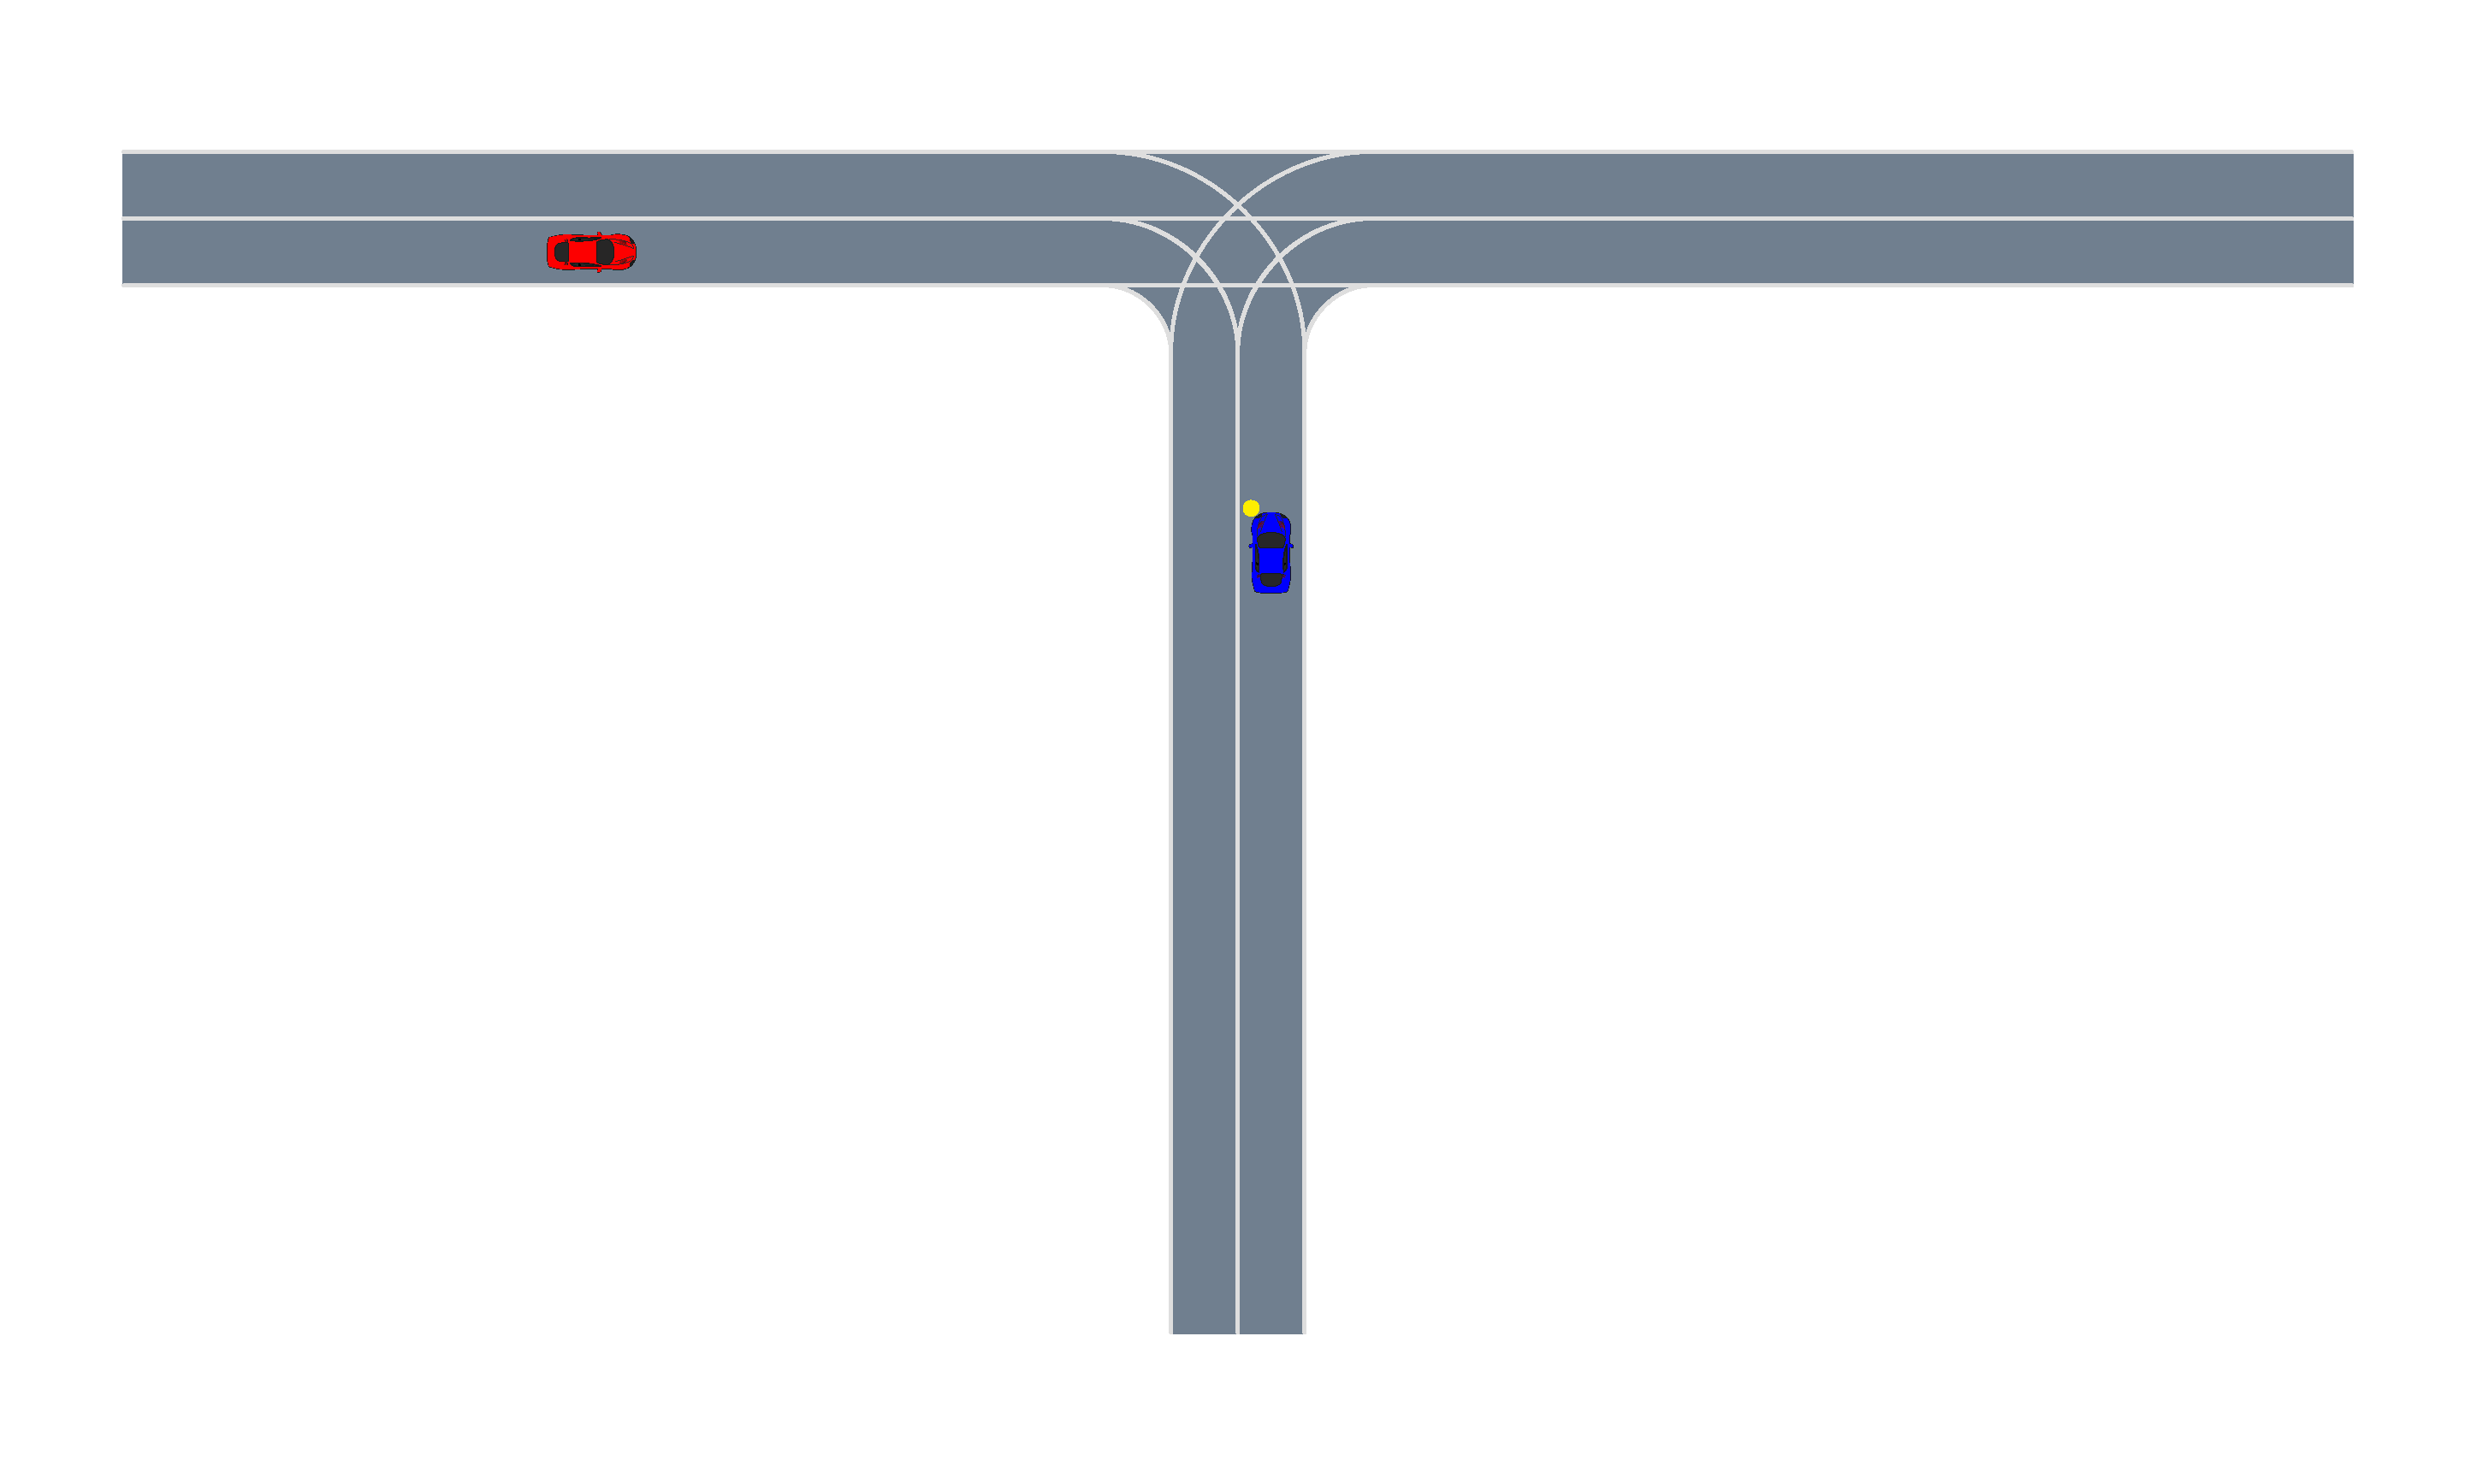
\includegraphics[width=0.9\textwidth, trim={10cm 16.5cm 22cm 0},clip]{figures/interpretable_validation/2car_res1_frame_01.pdf}
    \end{subfigure}%
   \begin{subfigure}[t]{0.33\columnwidth}
        \centering
        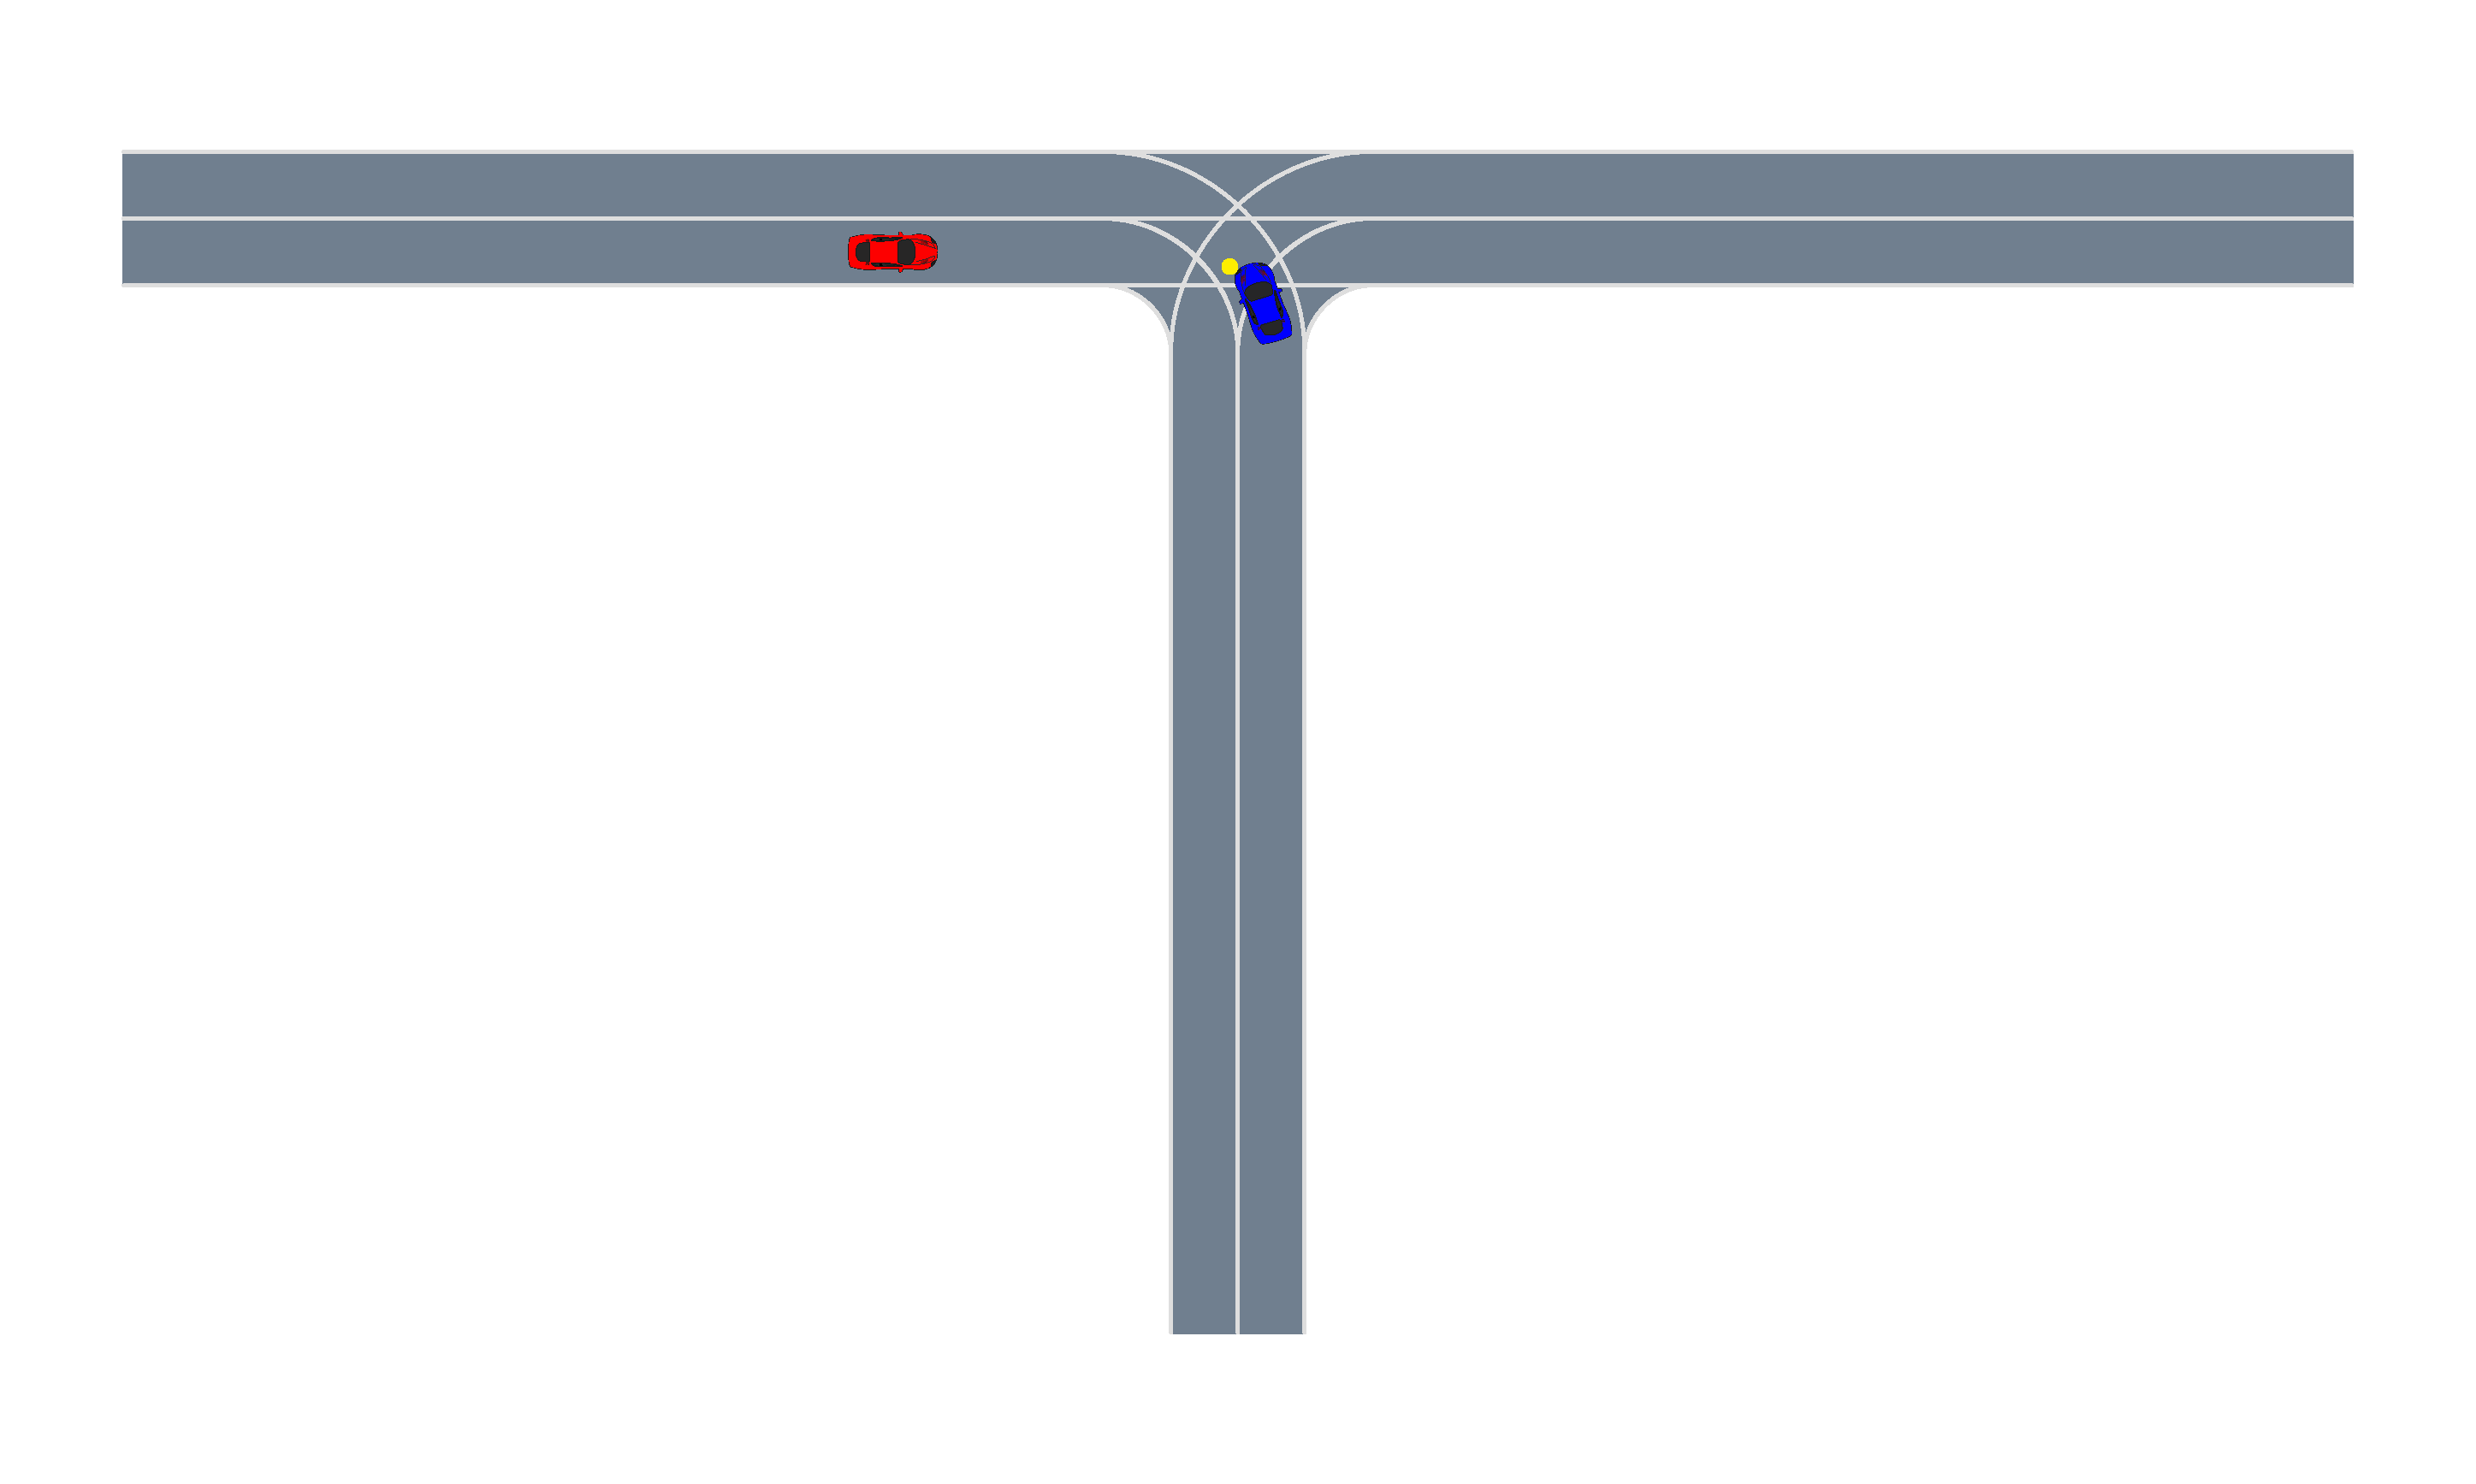
\includegraphics[width=0.9\textwidth, trim={10cm 16.5cm 22cm 0},clip]{figures/interpretable_validation/2car_res1_frame_07.pdf}
    \end{subfigure}%
    \begin{subfigure}[t]{0.33\columnwidth}
        \centering
        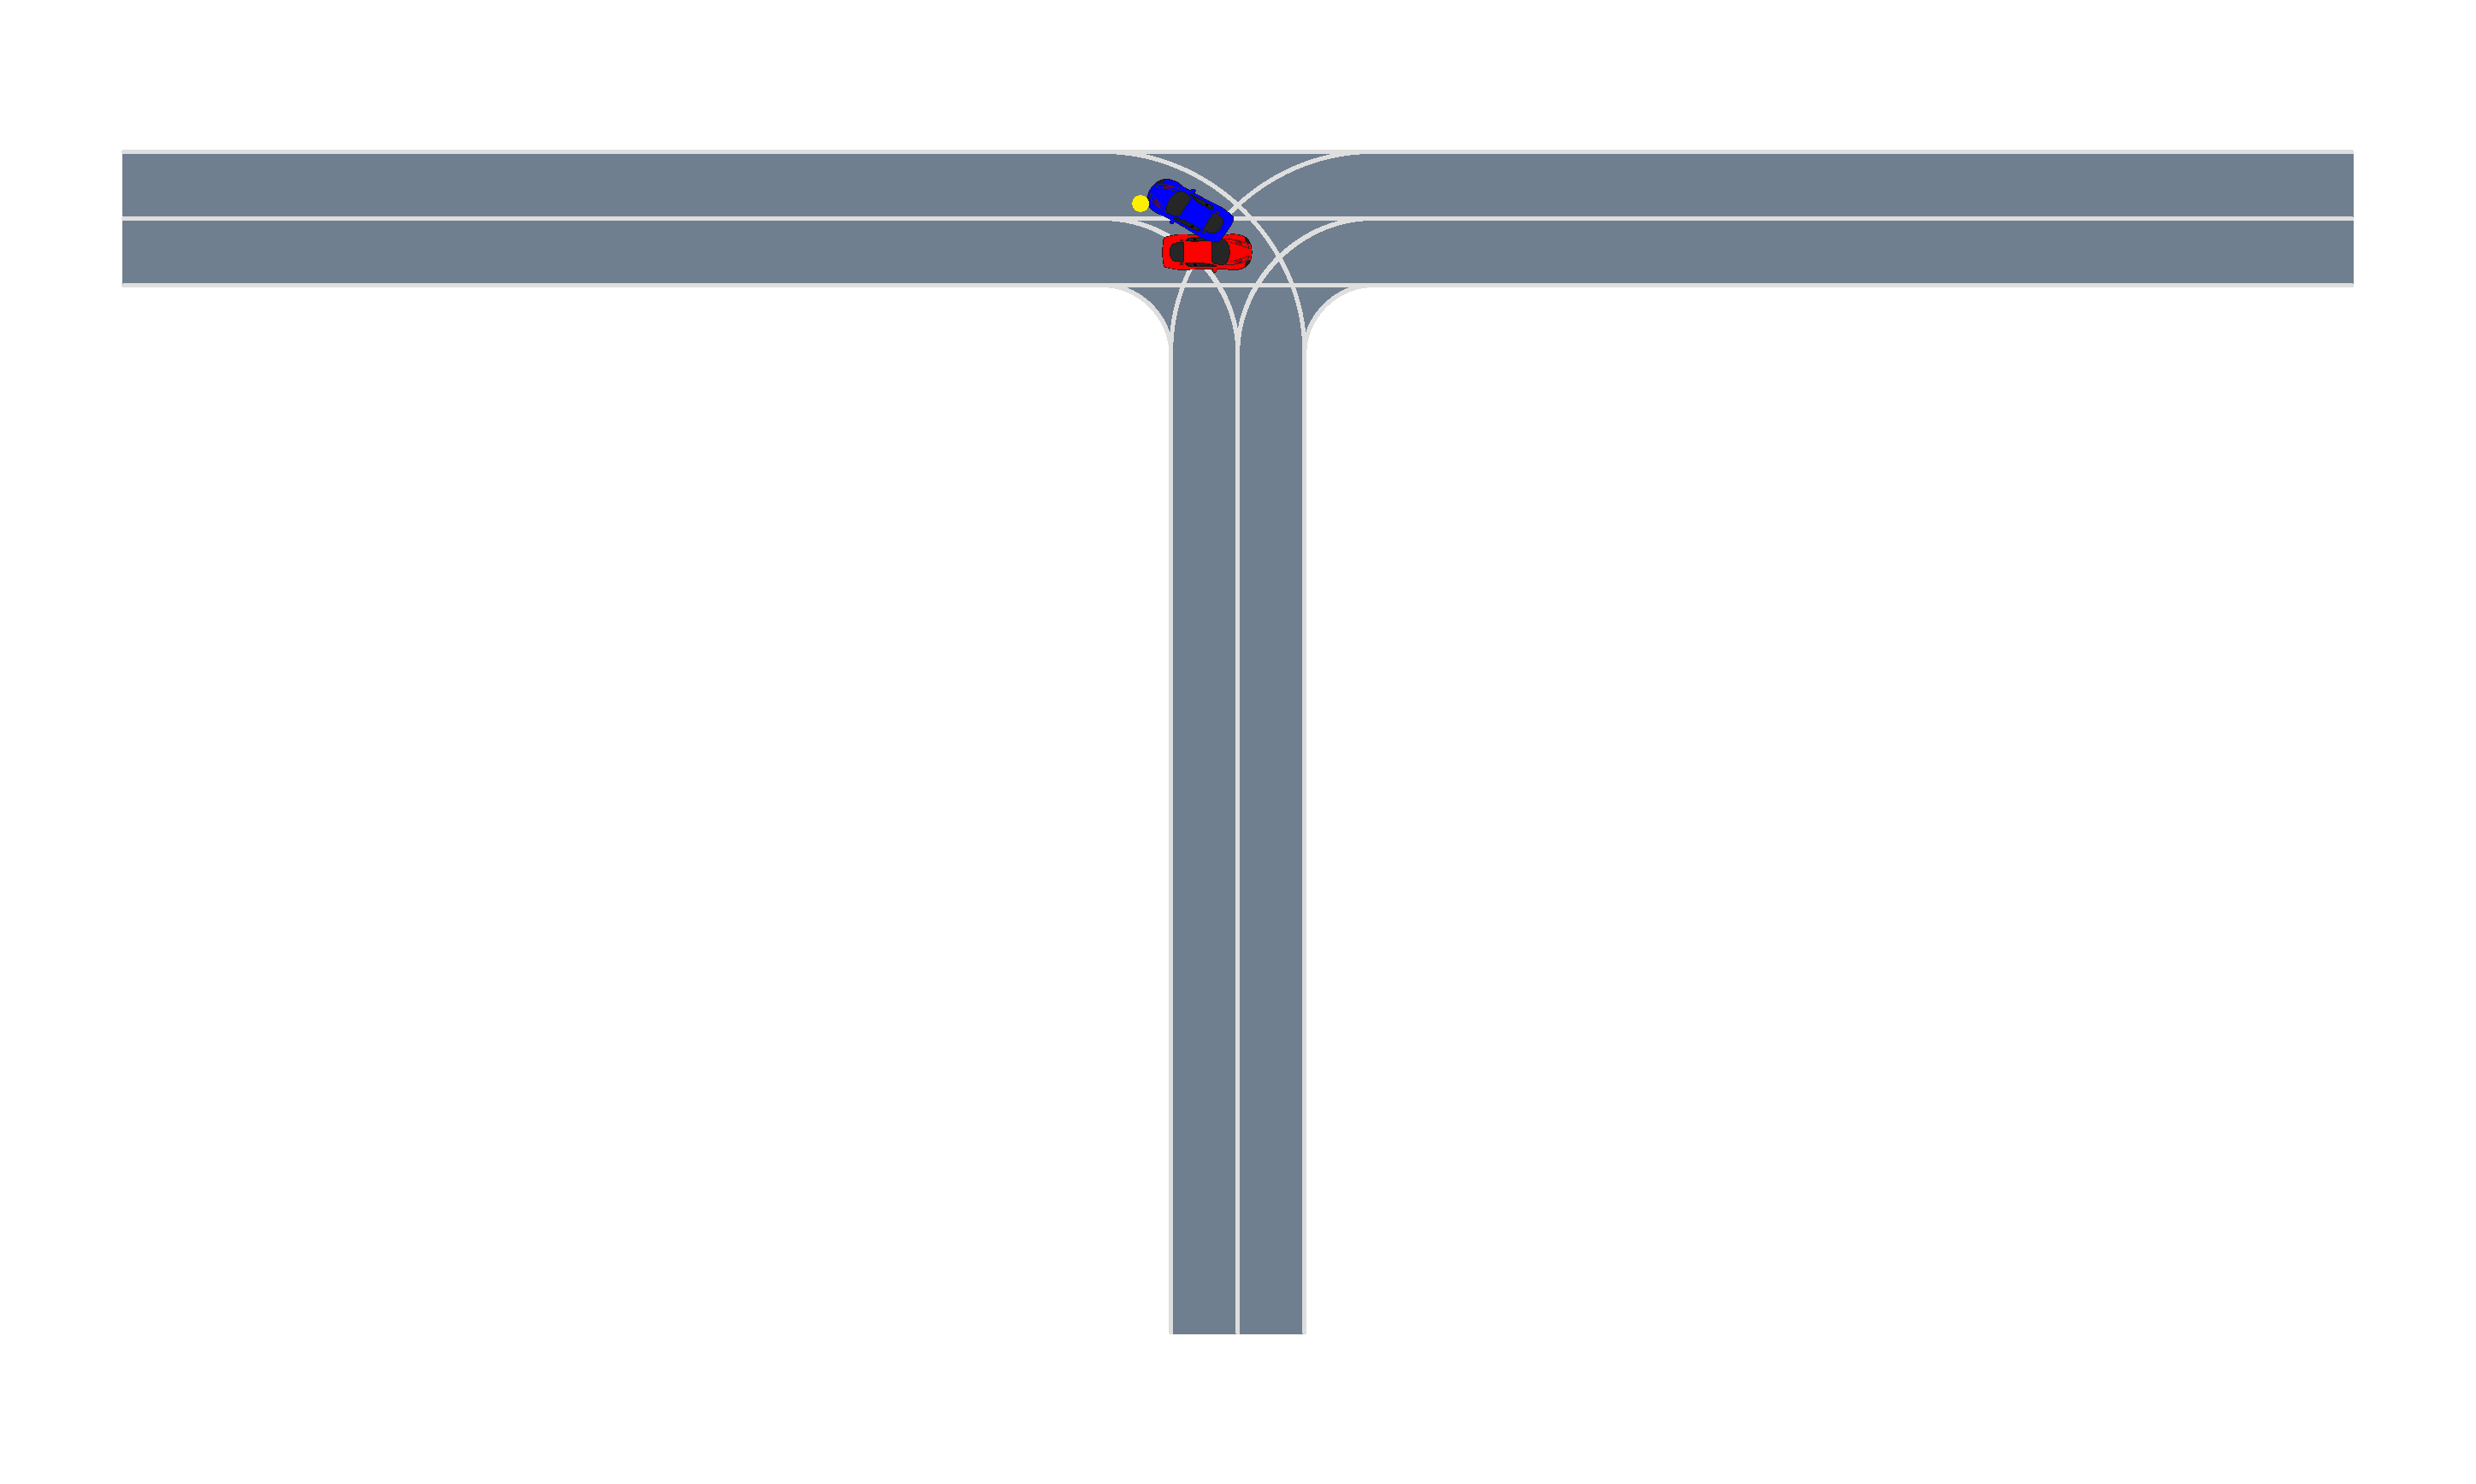
\includegraphics[width=0.9\textwidth, trim={10cm 16.5cm 22cm 0},clip]{figures/interpretable_validation/2car_res1_frame_12.pdf}
    \end{subfigure}
    \caption{Collision for LT1 at $t=(\SI{0}{s}, \SI{1.08}{s}, \SI{1.98}{s})$.}
    \label{fig:2car_LT1}
    \vskip -0.2in
\end{figure}


%%%% Second initial condition
\begin{figure}
    \centering
    \begin{subfigure}[t]{0.33\columnwidth}
        \centering
        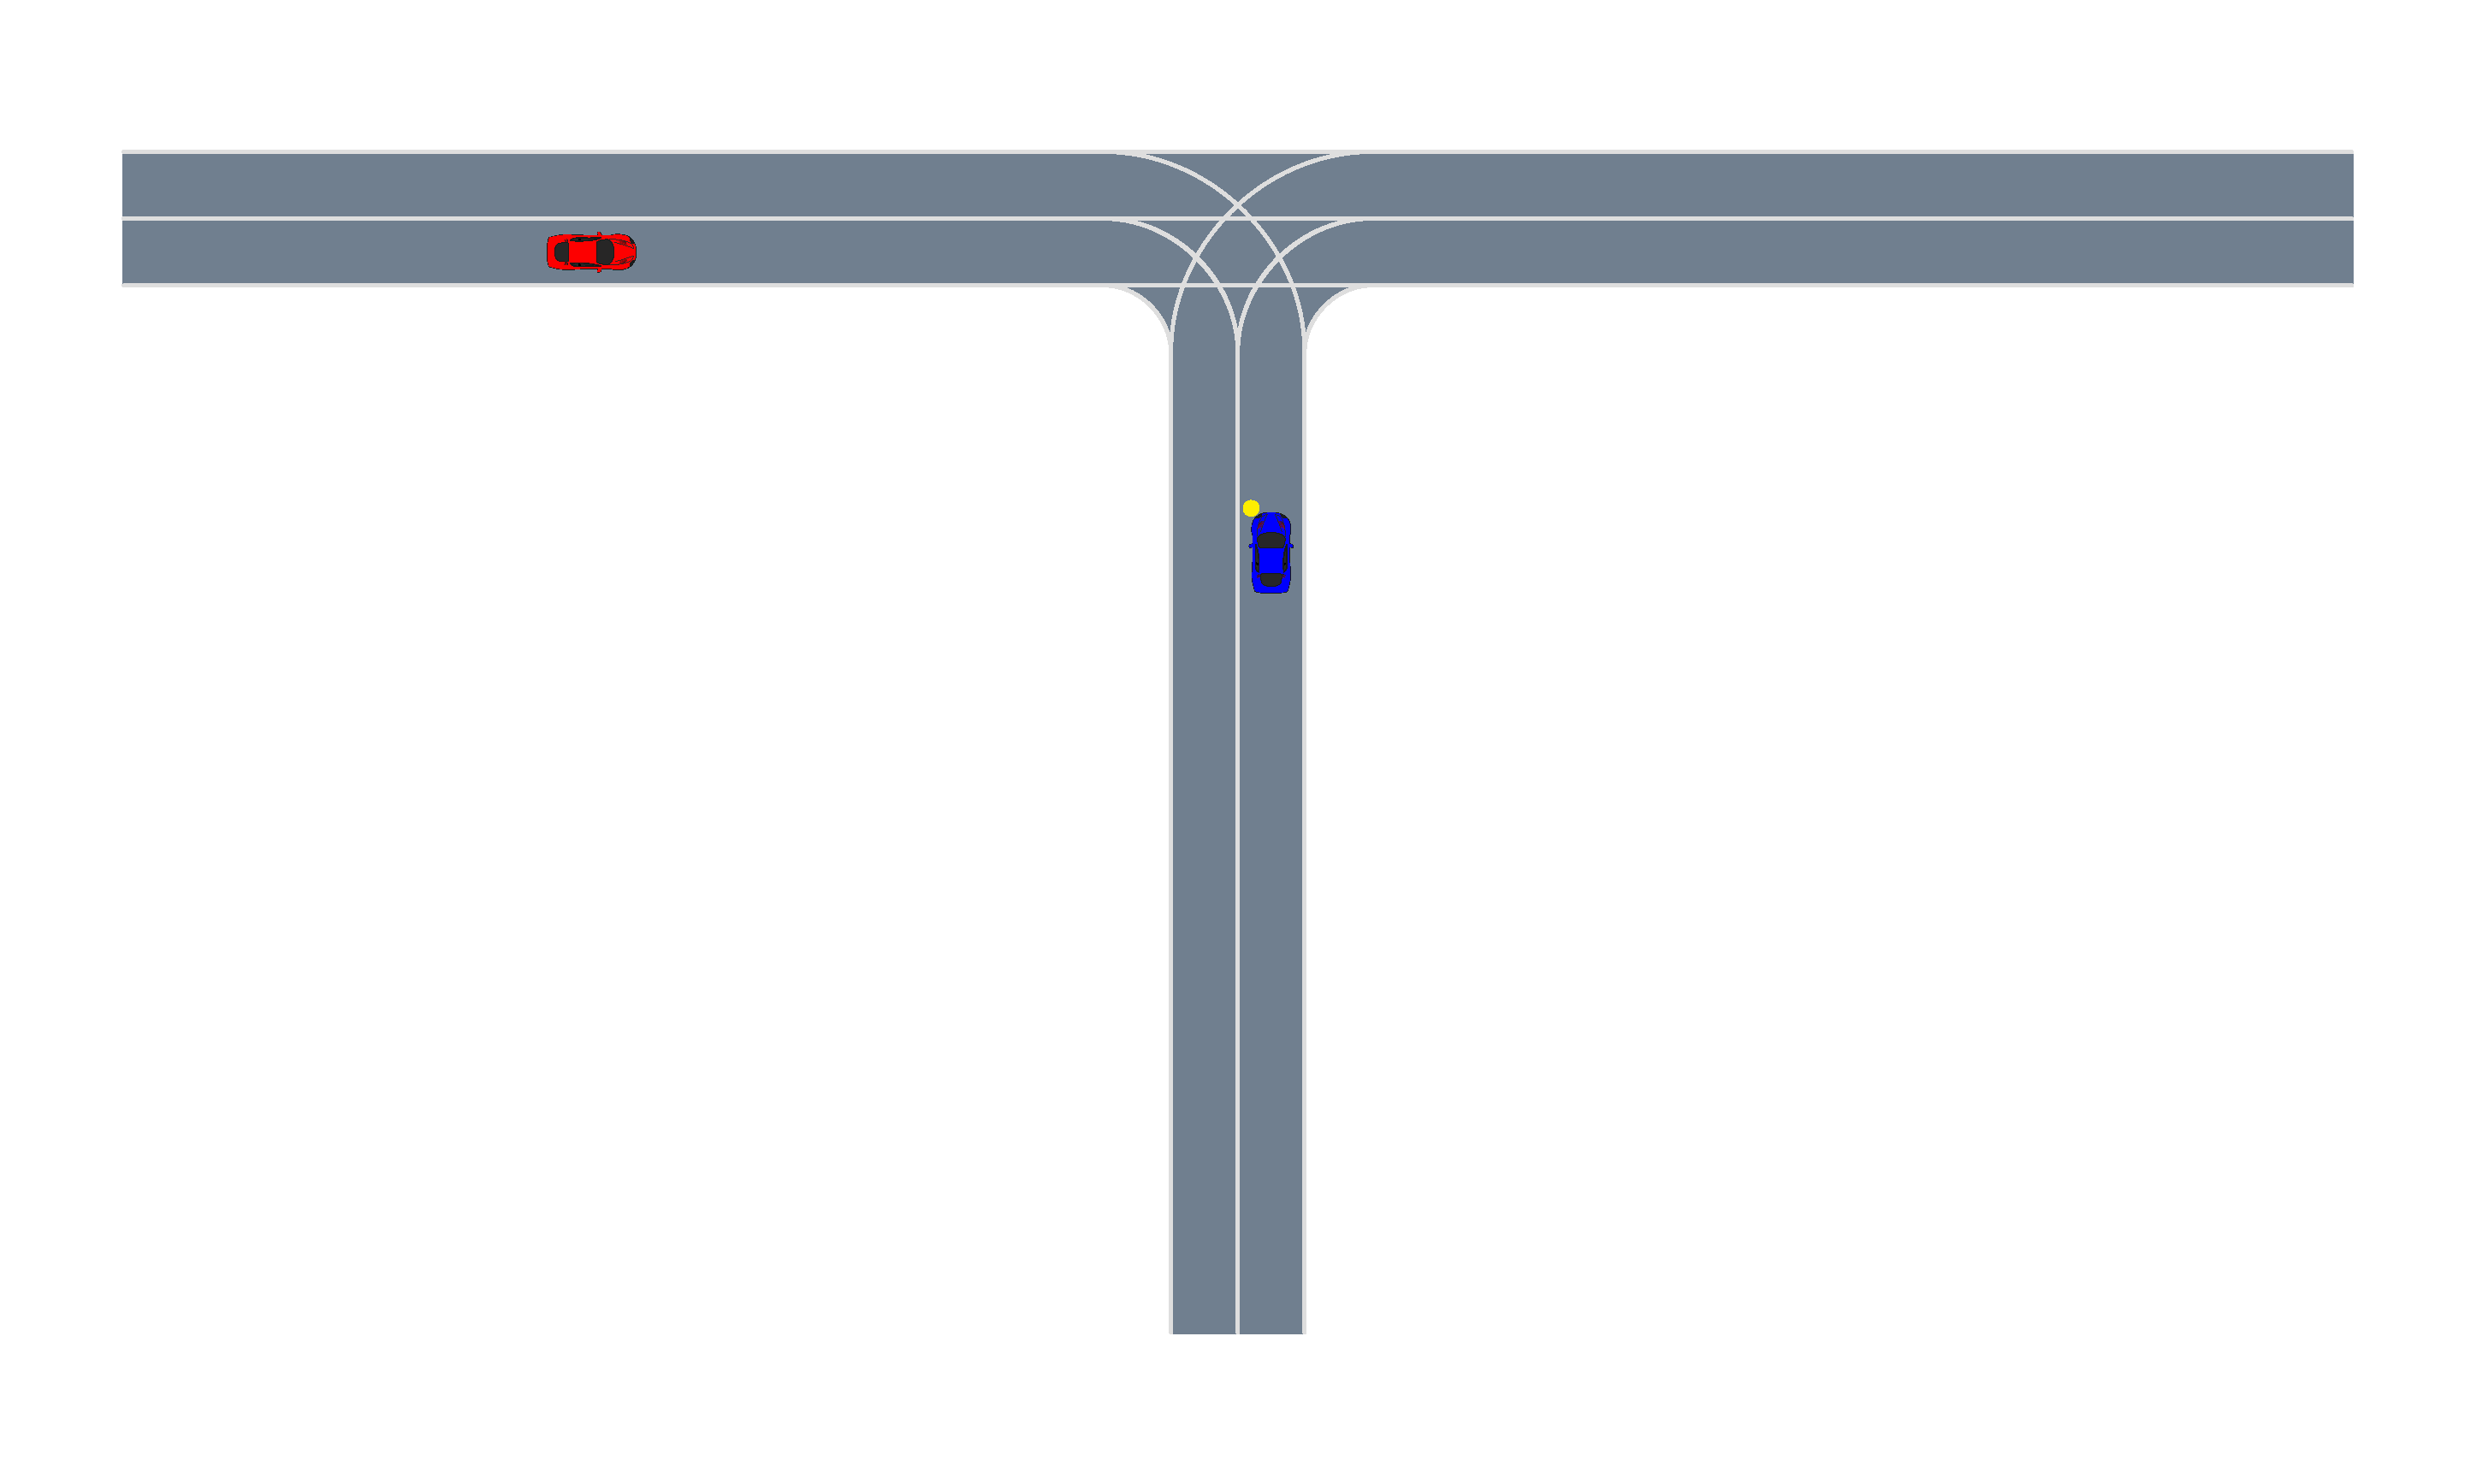
\includegraphics[width=0.9\textwidth, trim={10cm 16.5cm 22cm 0},clip]{figures/interpretable_validation/2car_res2_frame_01.pdf}
    \end{subfigure}%
   \begin{subfigure}[t]{0.33\columnwidth}
        \centering
        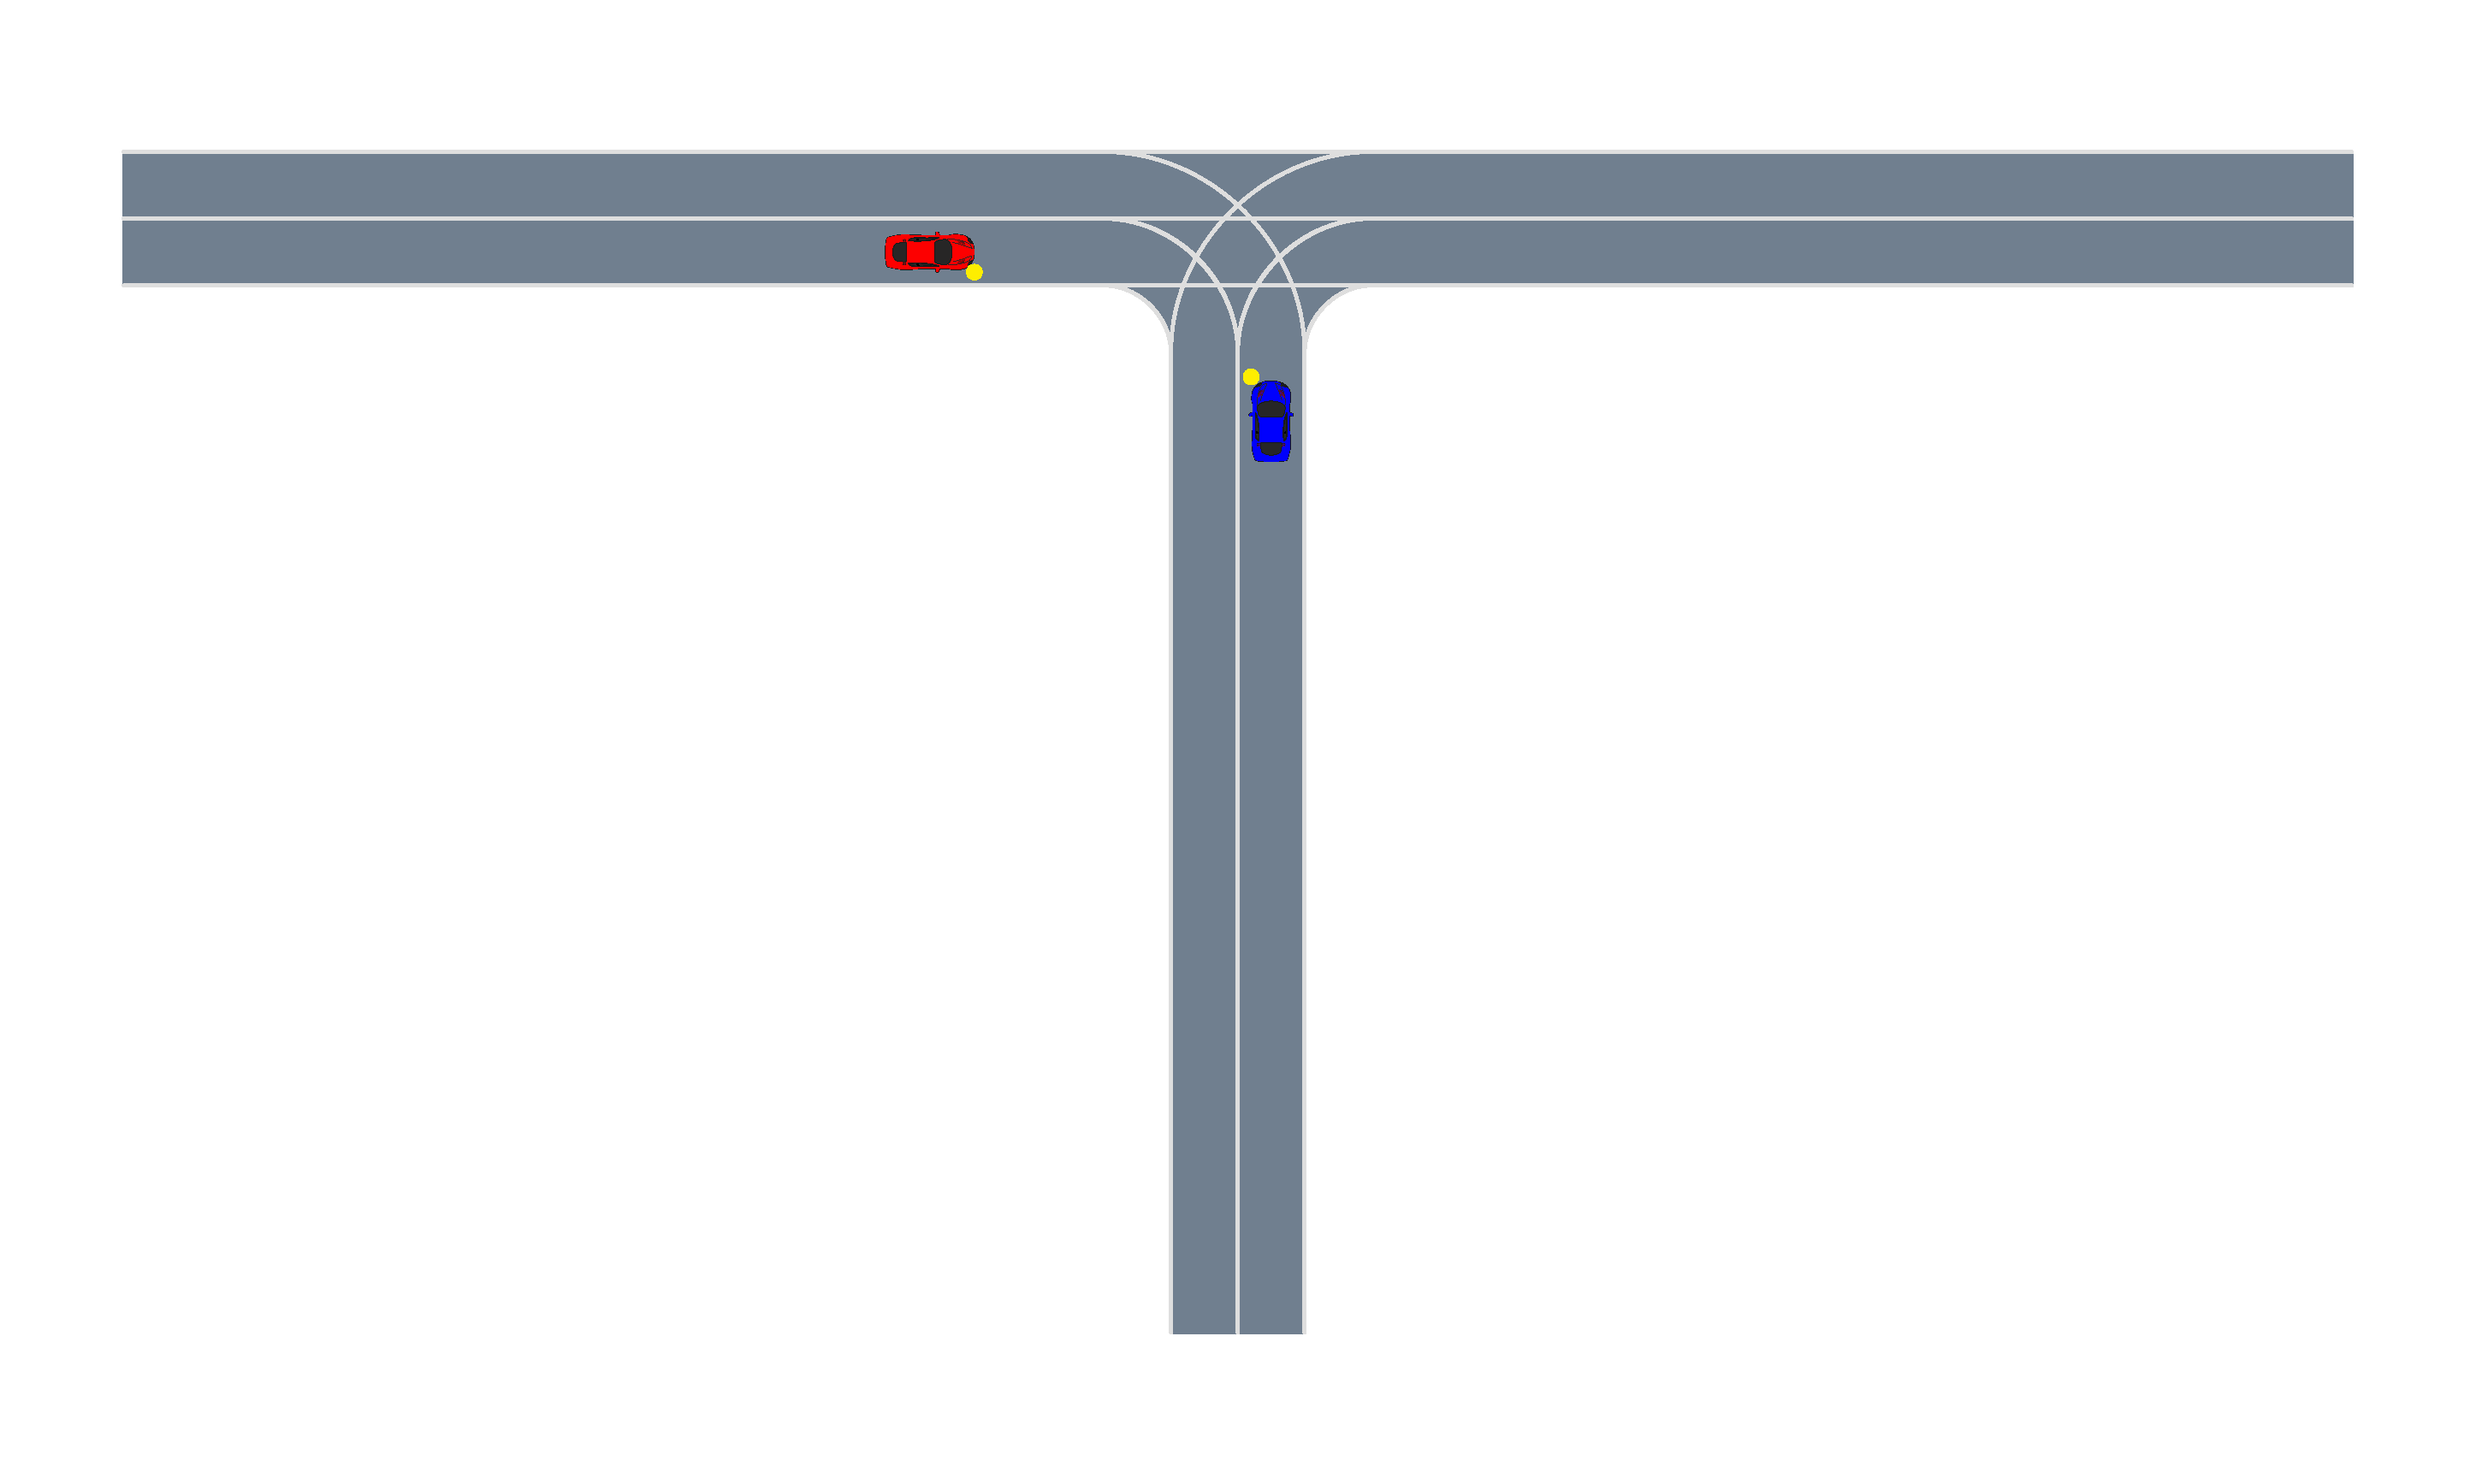
\includegraphics[width=0.9\textwidth, trim={10cm 16.5cm 22cm 0},clip]{figures/interpretable_validation/2car_res2_frame_05.pdf}
    \end{subfigure}%
    \begin{subfigure}[t]{0.33\columnwidth}
        \centering
        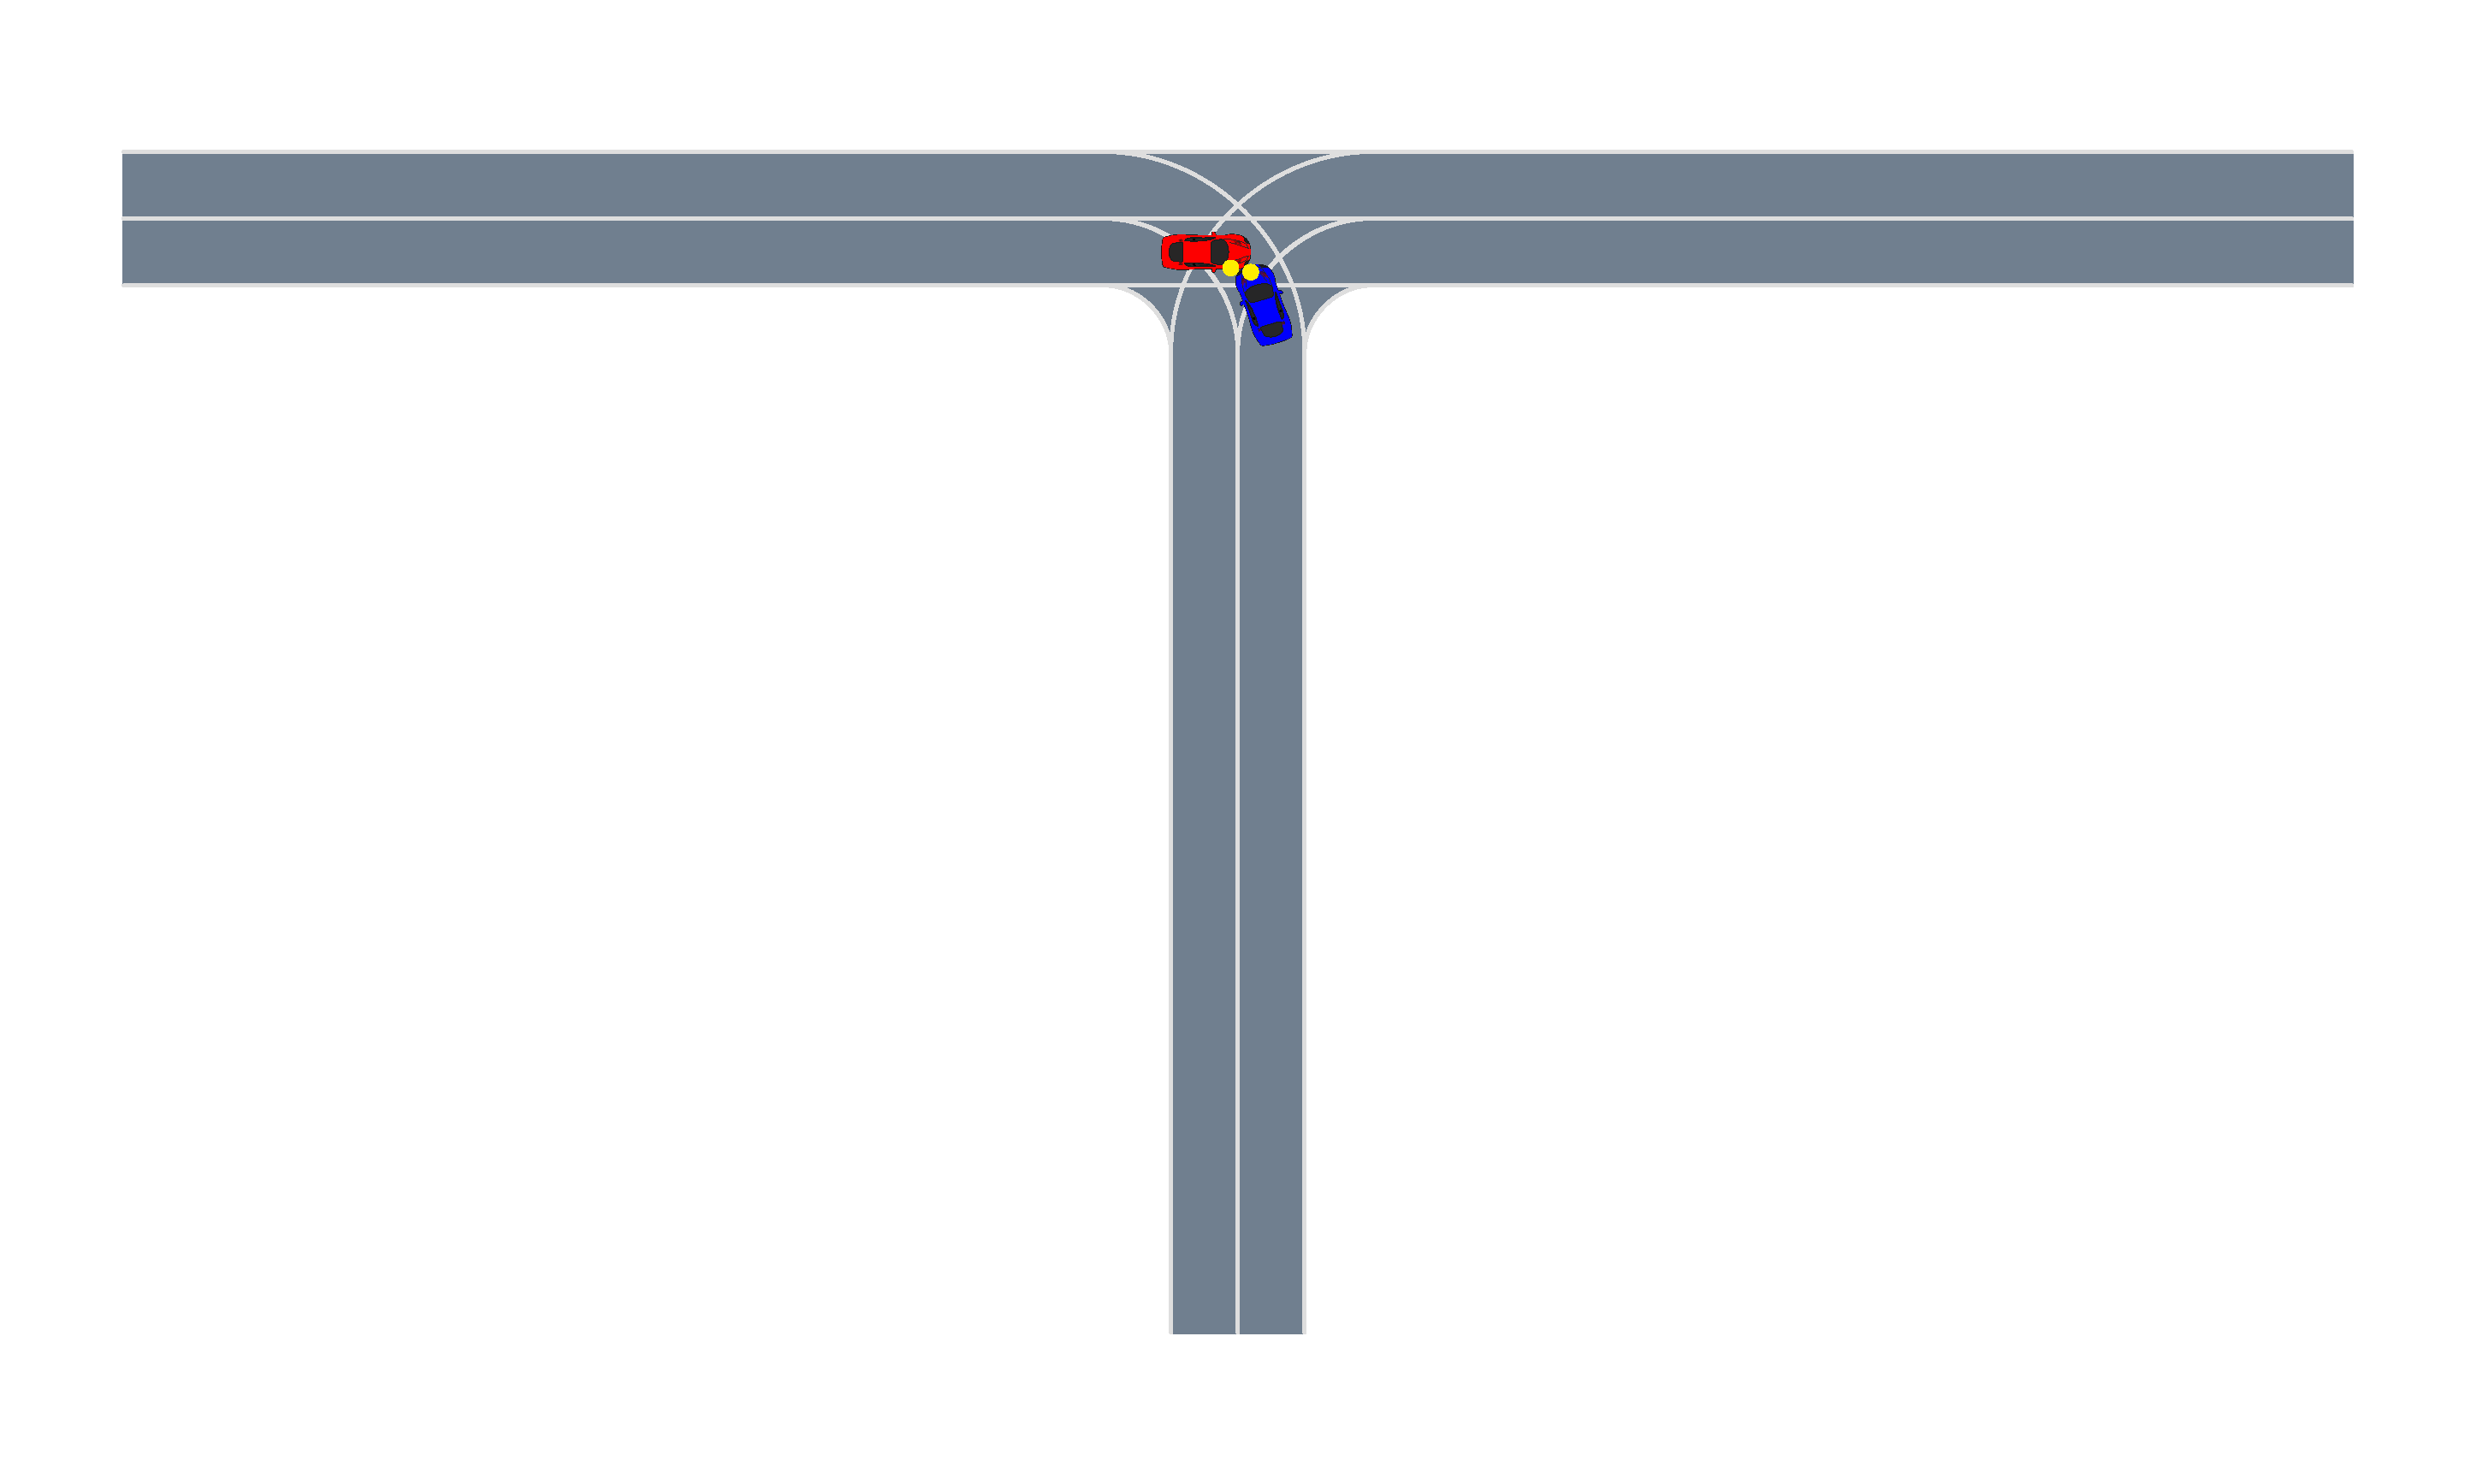
\includegraphics[width=0.9\textwidth, trim={10cm 16.5cm 22cm 0},clip]{figures/interpretable_validation/2car_res2_frame_08.pdf}
    \end{subfigure}
    \caption{Collision for LT2 at $t=(\SI{0}{s}, \SI{0.72}{s}, \SI{1.26}{s})$.}
    \label{fig:2car_LT2}
    \vskip -0.2in
\end{figure}


%%% Third initial condition
\begin{figure}
\vskip -0.2in
    \centering
    \begin{subfigure}[t]{0.33\columnwidth}
        \centering
        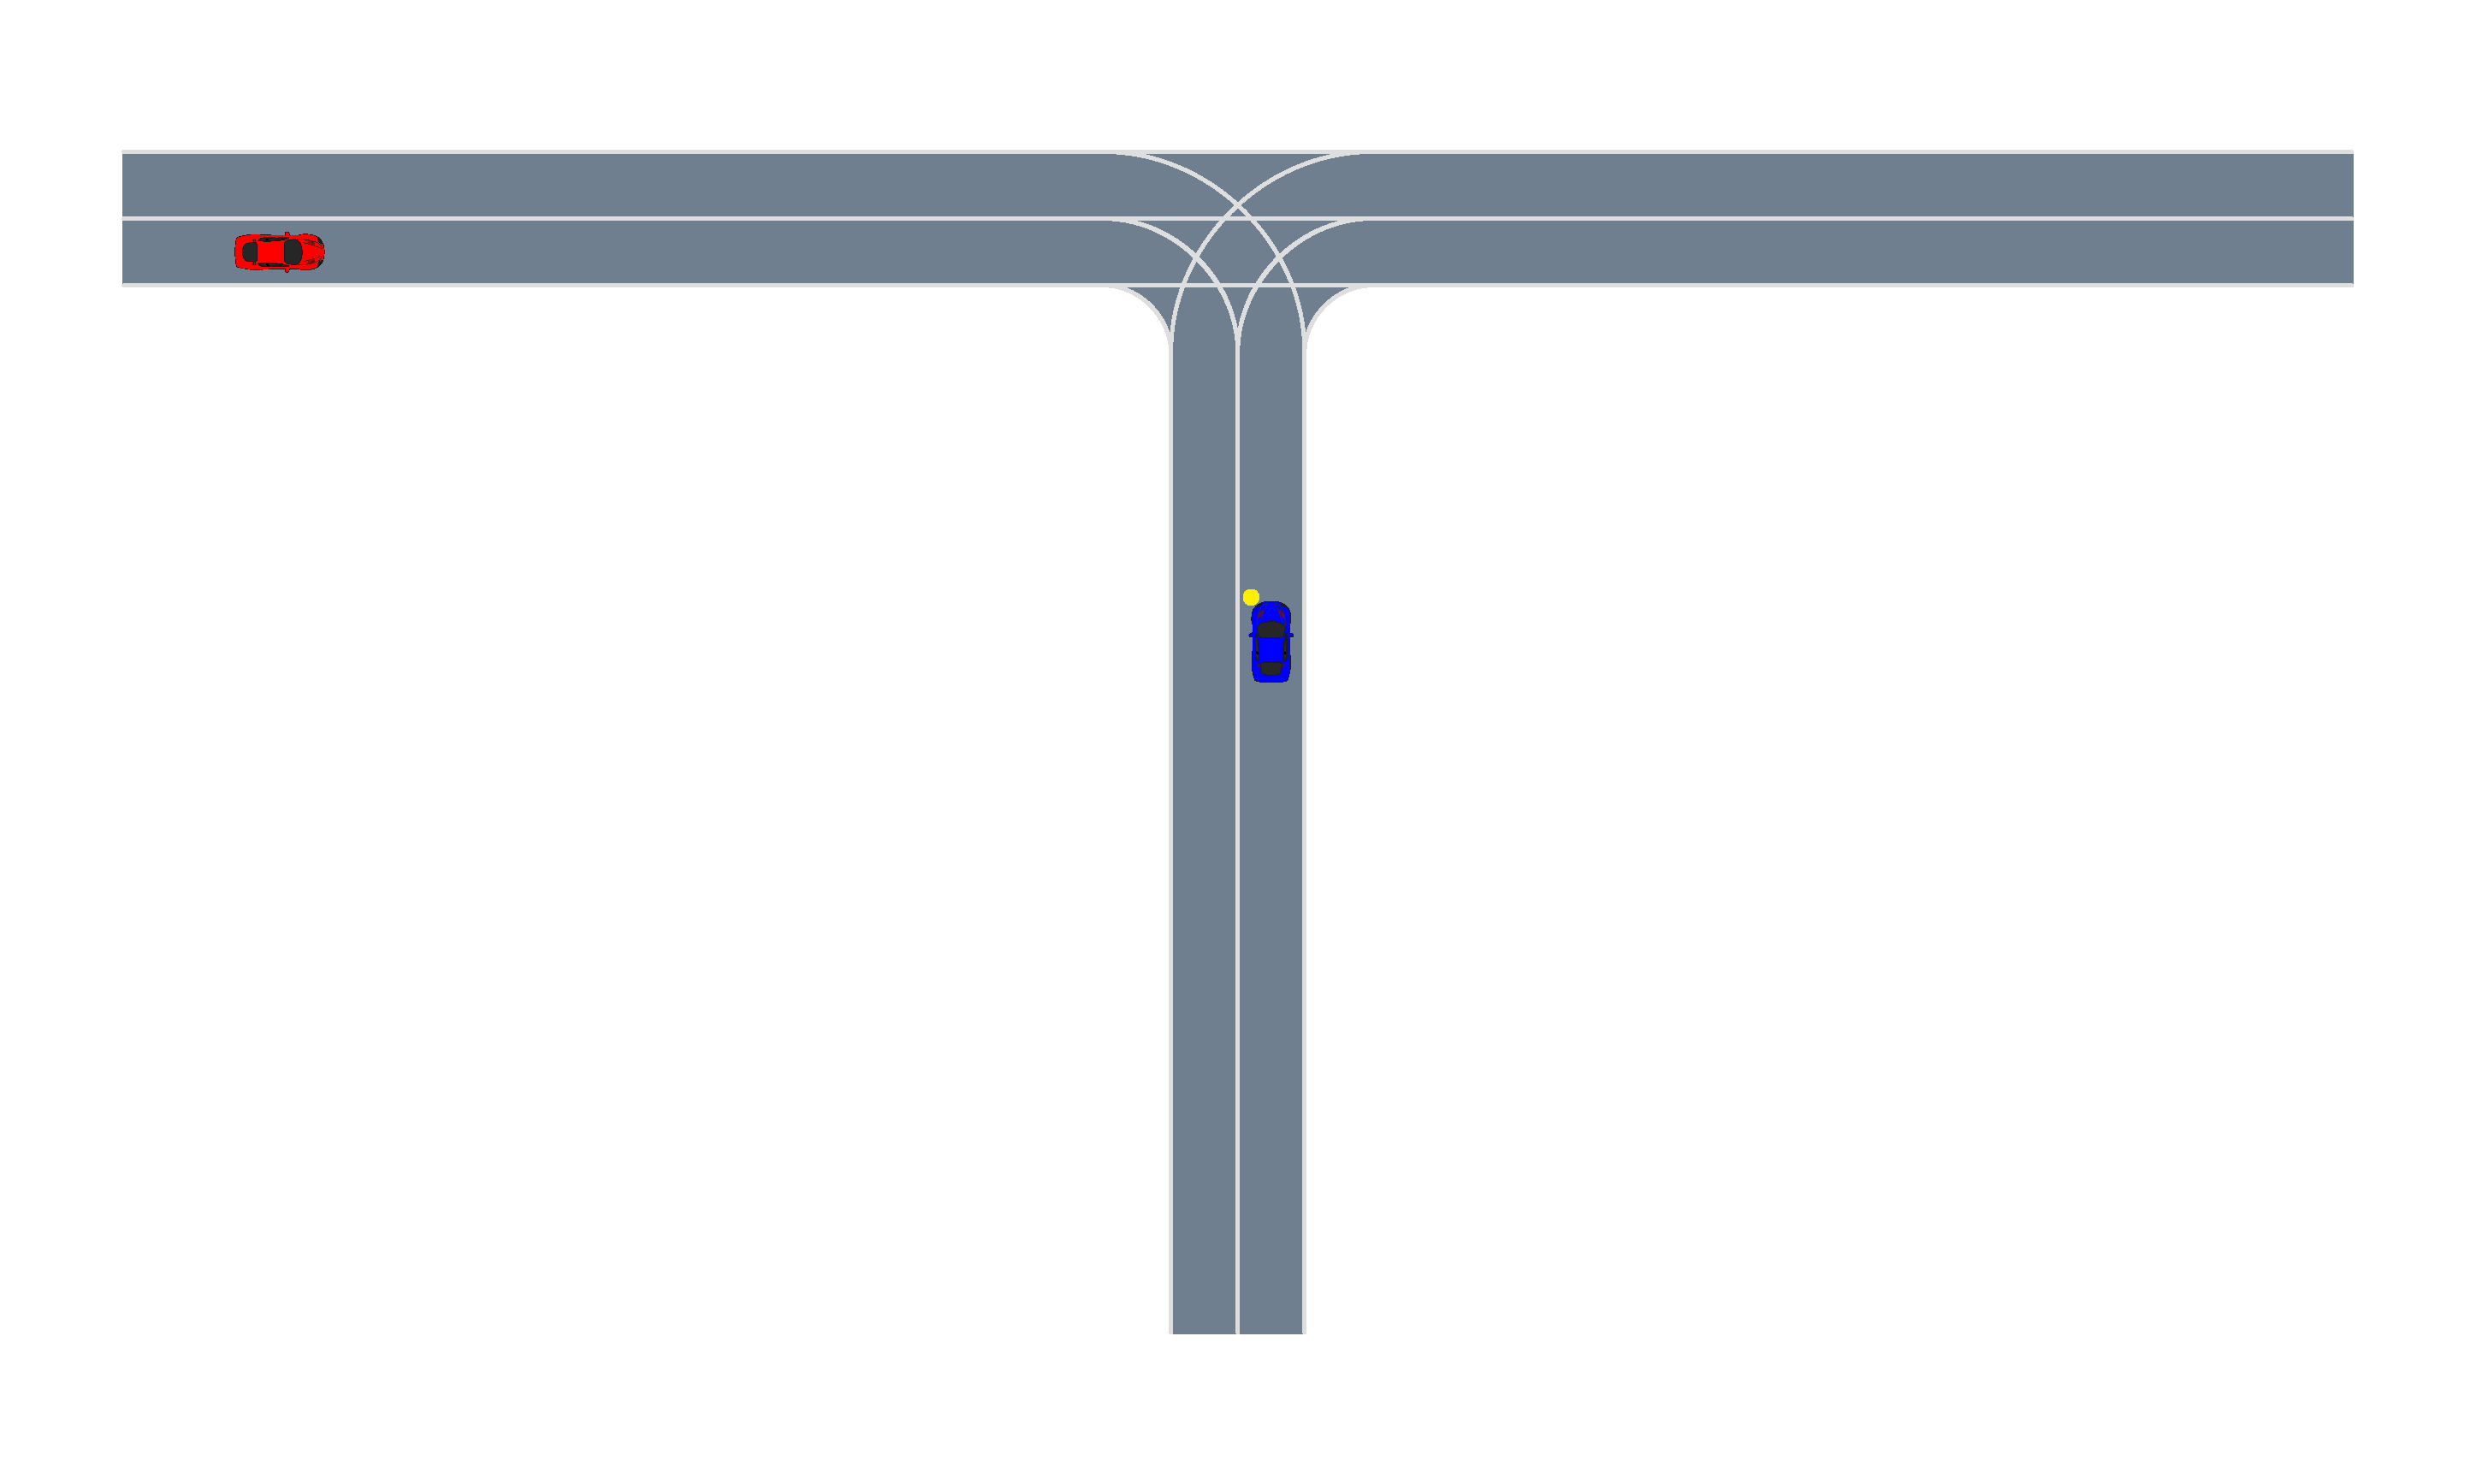
\includegraphics[width=0.9\textwidth, trim={8cm 16cm 22cm 0},clip]{figures/interpretable_validation/2car_res3_frame_01.pdf}
    \end{subfigure}%
   \begin{subfigure}[t]{0.33\columnwidth}
        \centering
        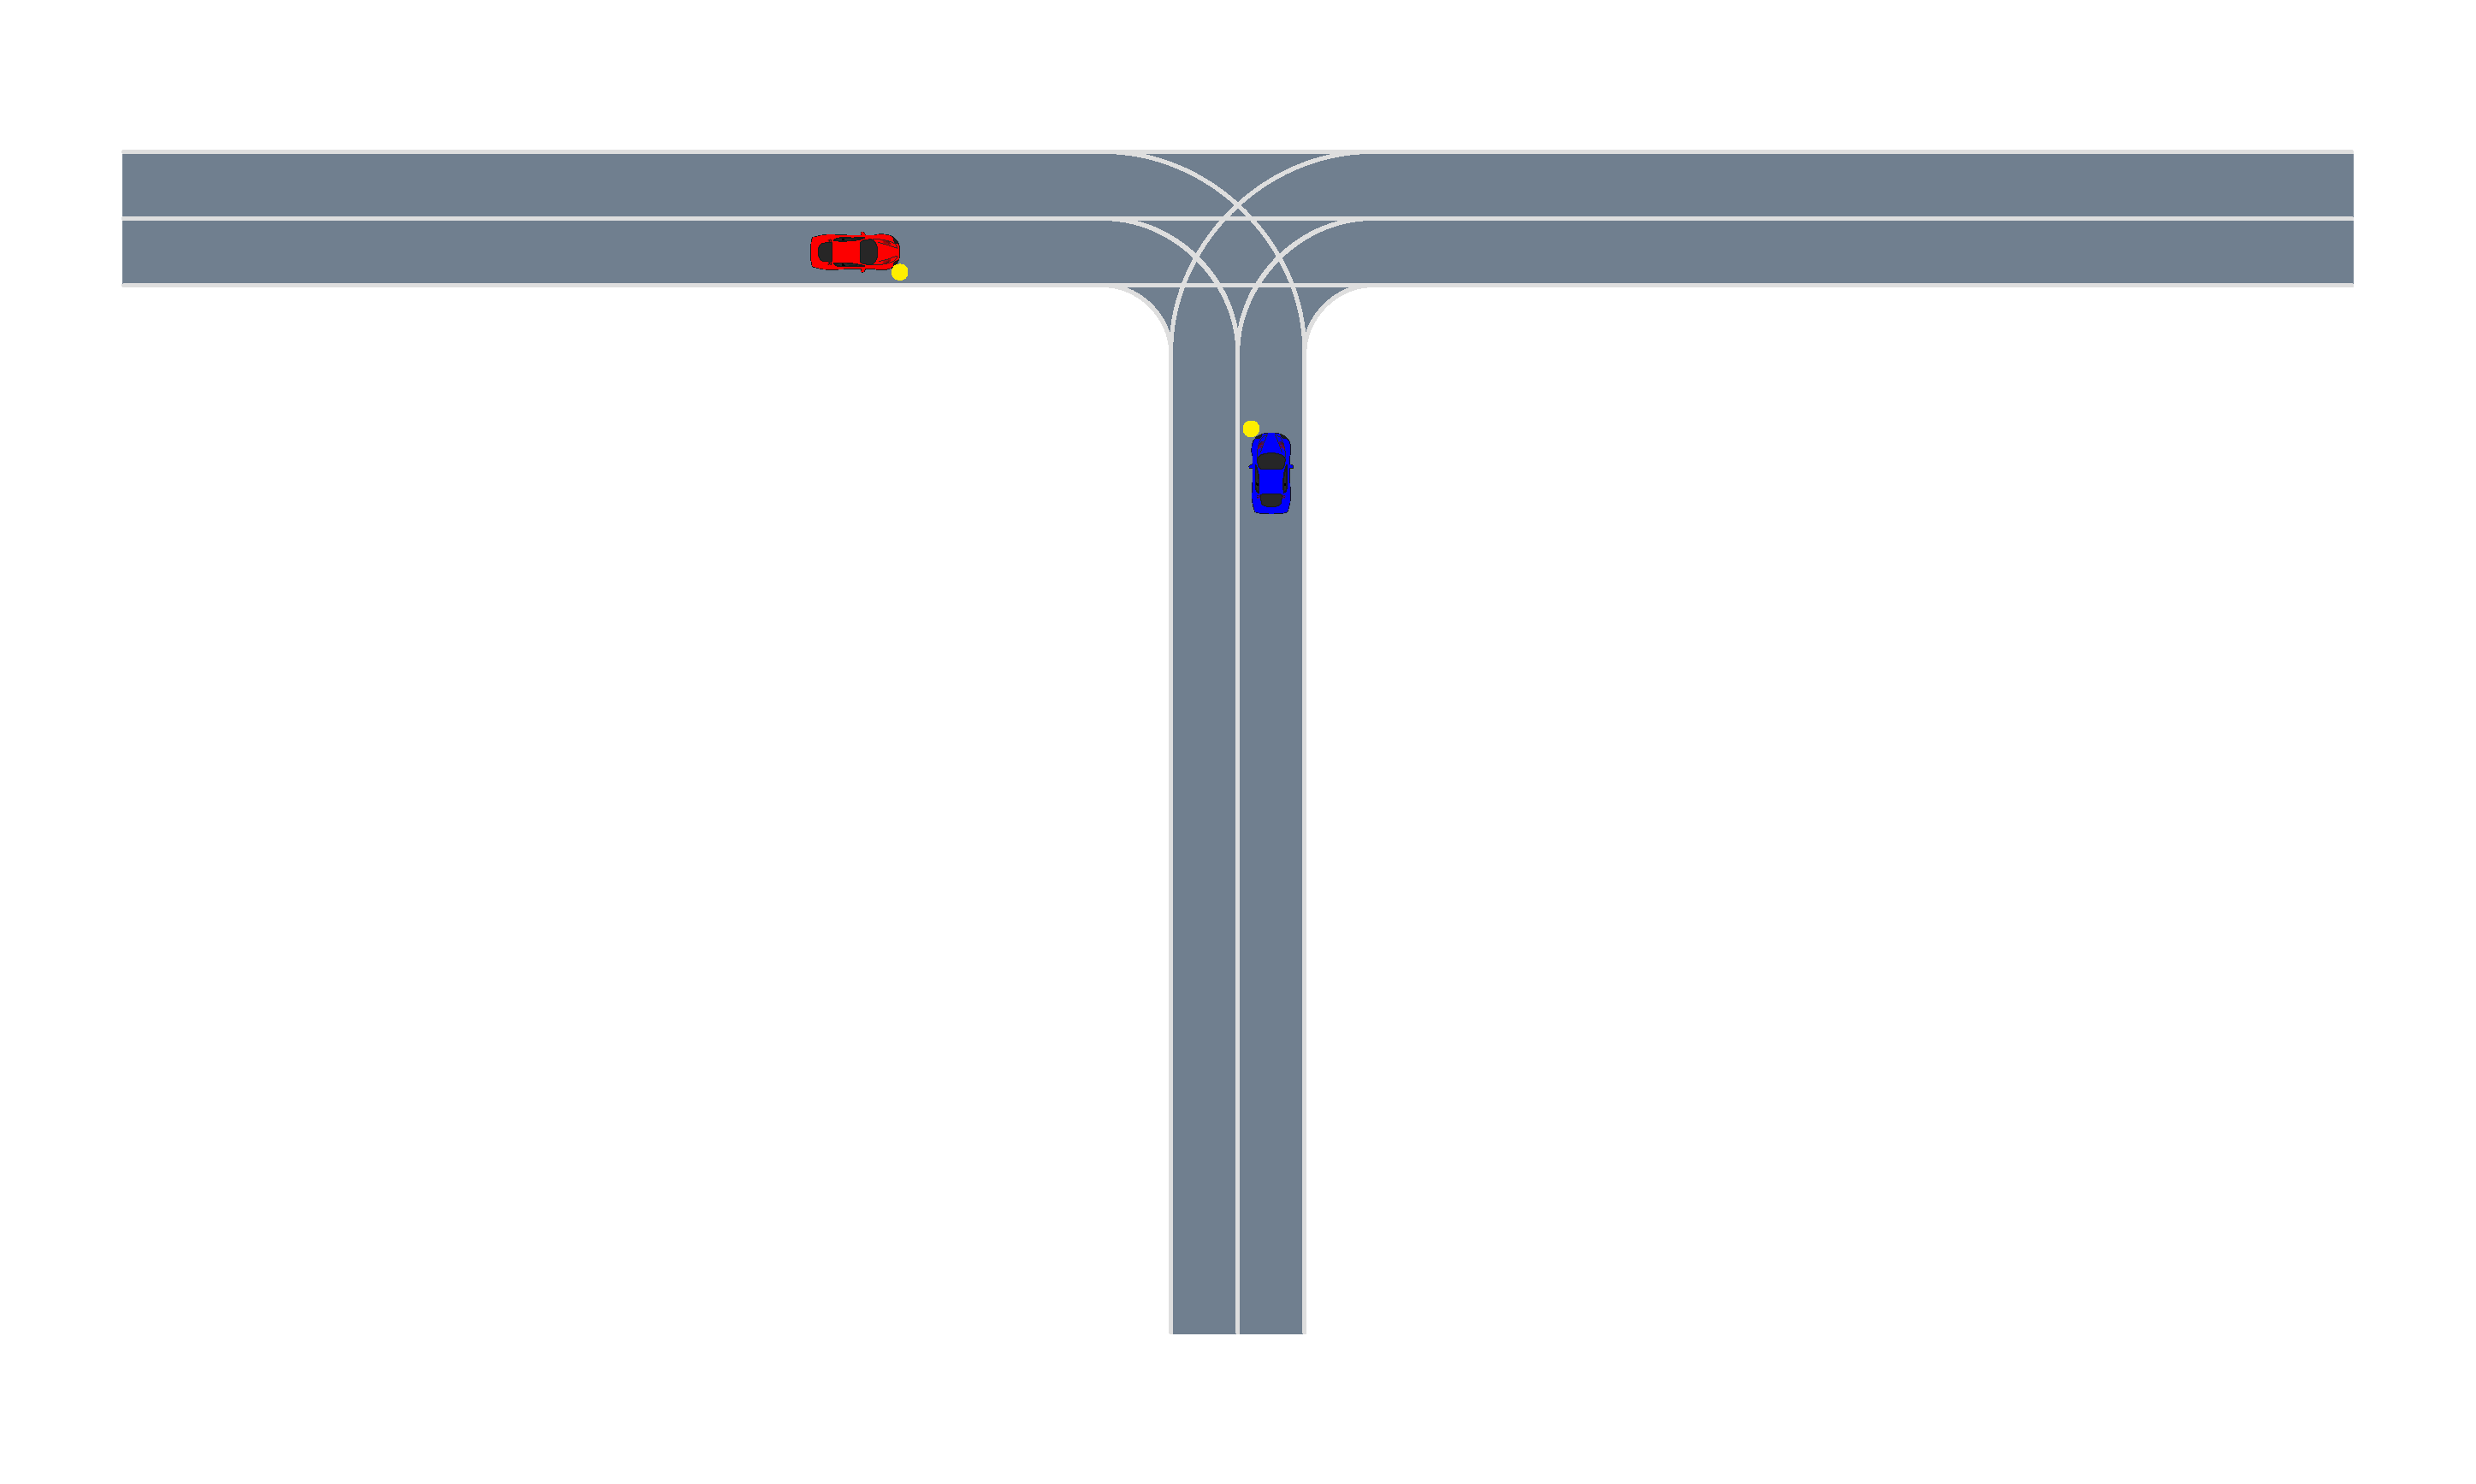
\includegraphics[width=0.9\textwidth, trim={10cm 16.5cm 22cm 0},clip]{figures/interpretable_validation/2car_res3_frame_06.pdf}
    \end{subfigure}%
    \begin{subfigure}[t]{0.33\columnwidth}
        \centering
        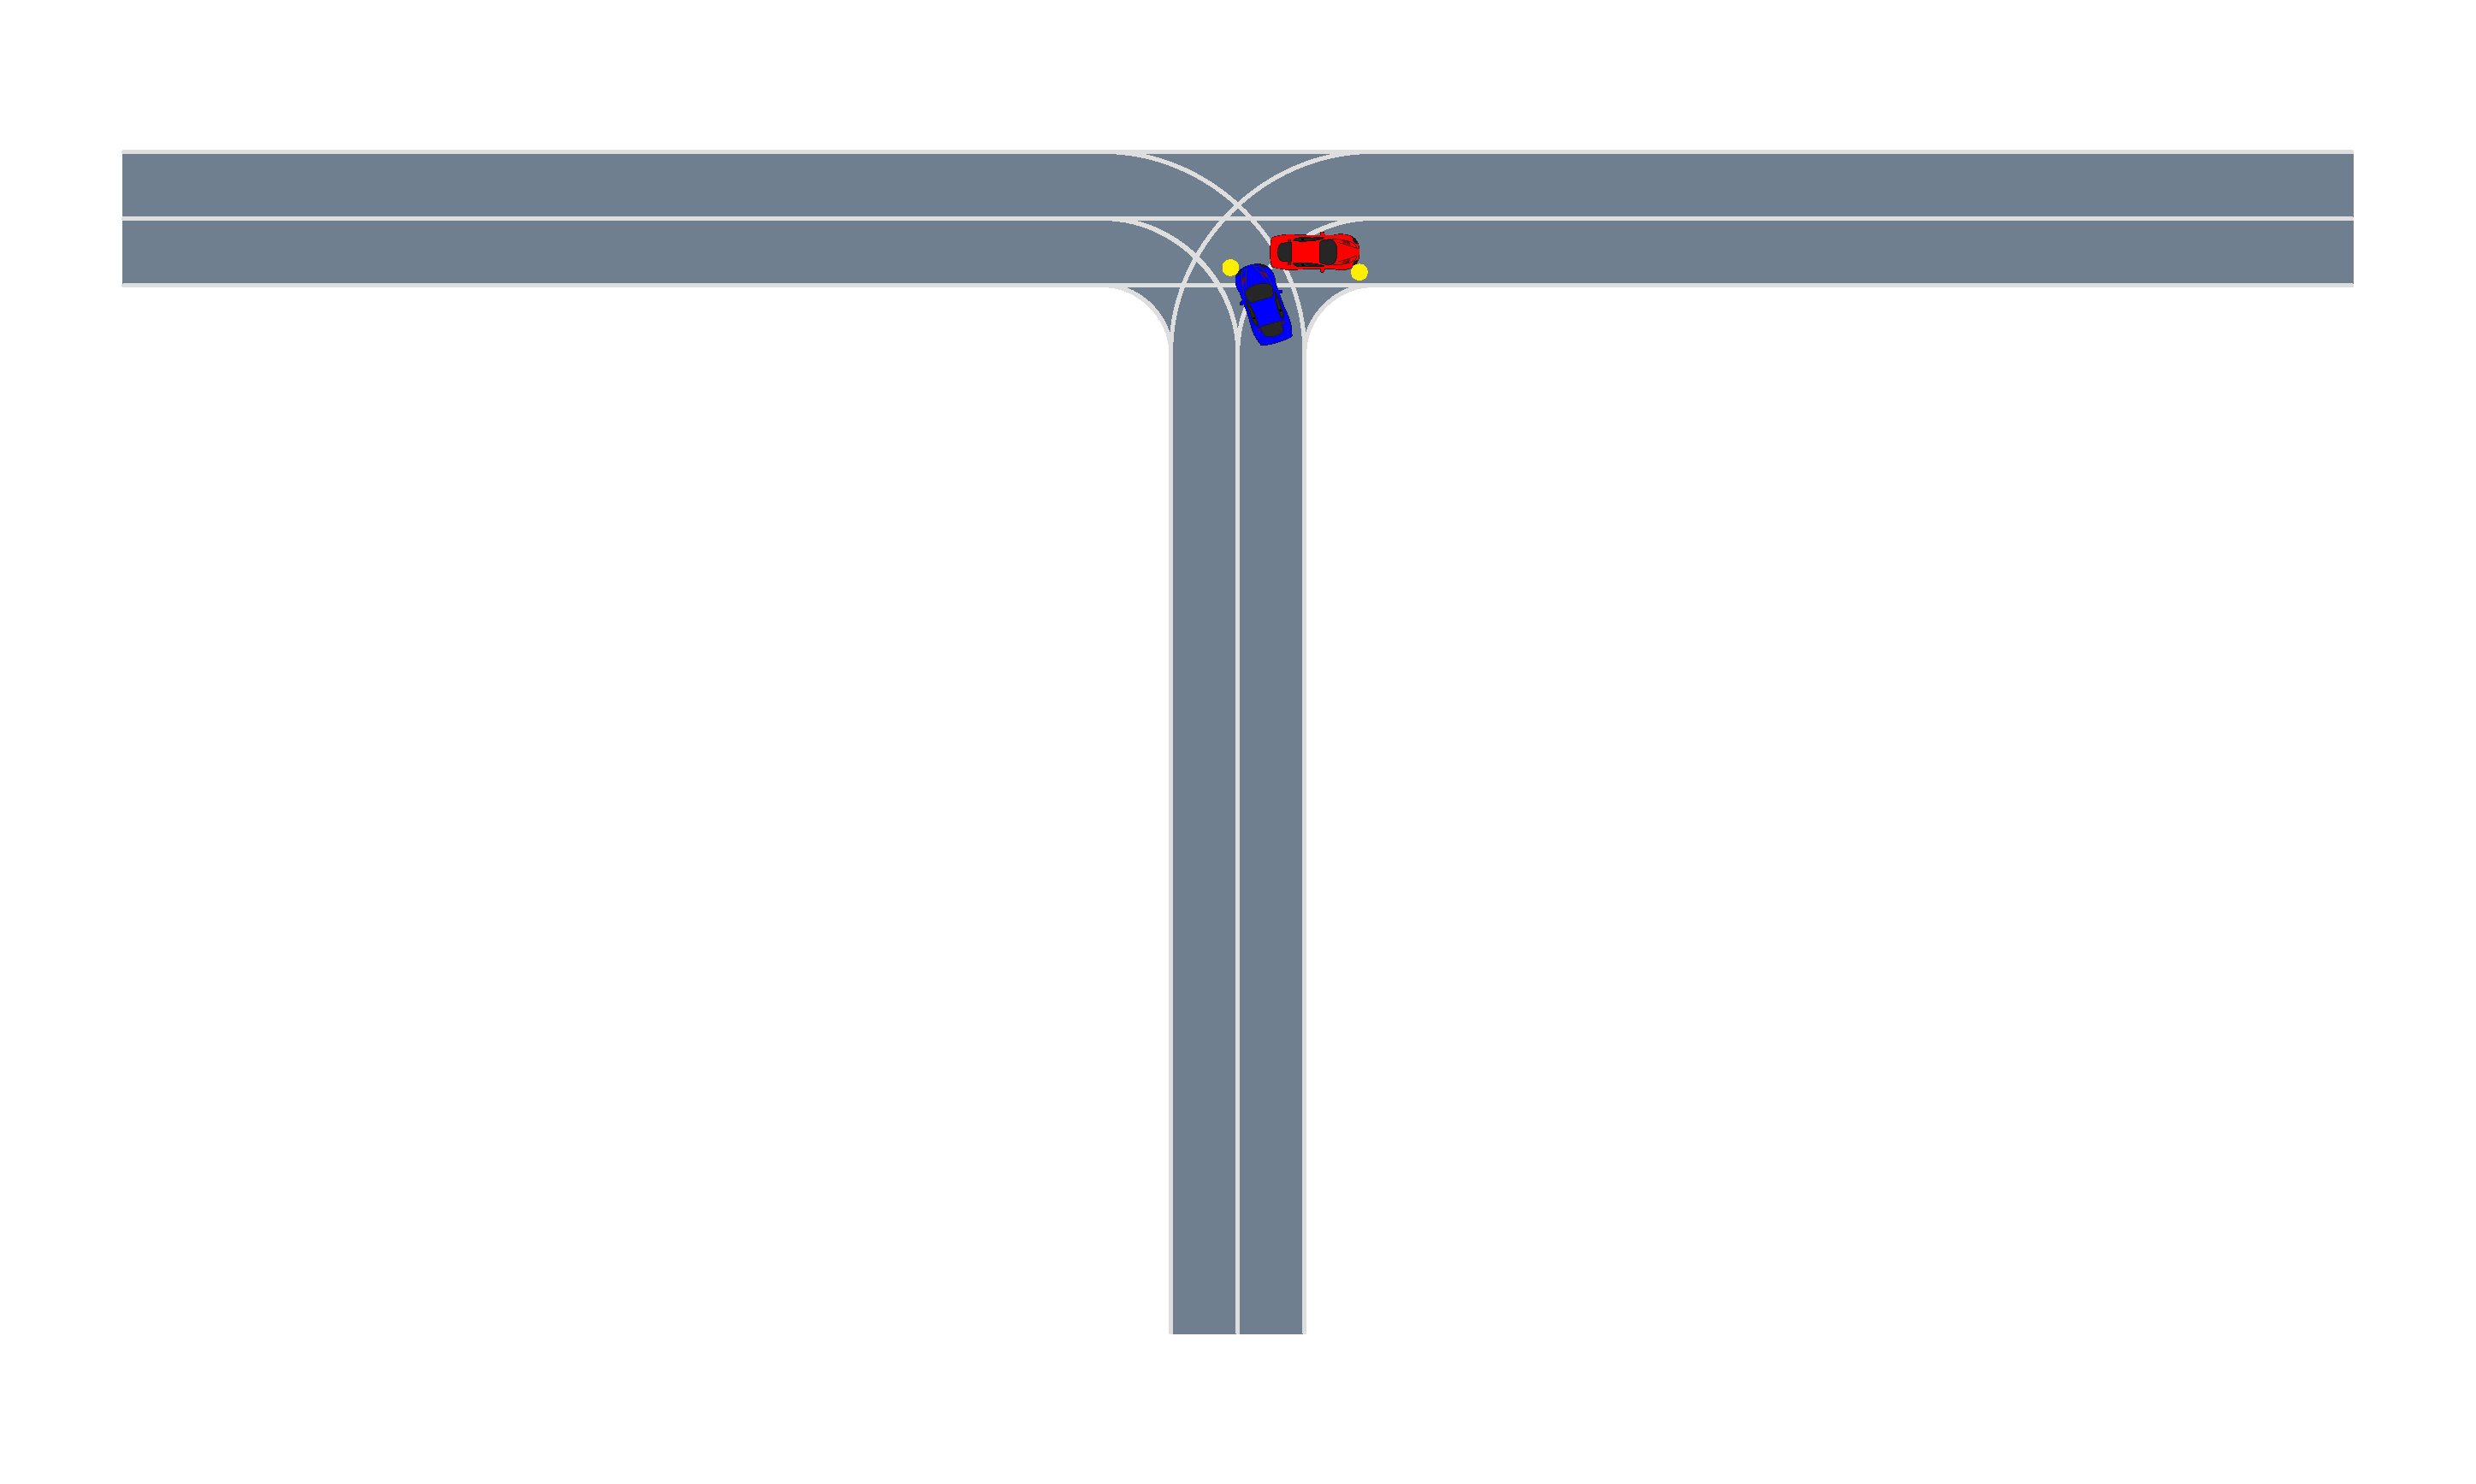
\includegraphics[width=0.9\textwidth, trim={10cm 16.5cm 22cm 0},clip]{figures/interpretable_validation/2car_res3_frame_10.pdf}
    \end{subfigure}
    \caption{Collision for LT3 at $t=(\SI{0}{s}, \SI{0.90}{s}, \SI{1.62}{s})$.}
    \label{fig:2car_LT3}
\end{figure}

% Sampling failure examples
One benefit to learning a failure description is the ability to produce many failure examples that have a shared temporal property. For example, we took the third failure description
\begin{equation}
    \square_{[0, .36]} B \lor d_{\rm maj}
\end{equation}
and use it to sample \num{10} failure trajectores. We plot the velocity vs. the position of the adversary for the failure examples in \cref{fig:2car_failure_samples}. We see that in the first two timesteps there is always a signification slowdown, but the trajectories then evolve stochastically before ending in a failure. 

\begin{figure}
    \centering
    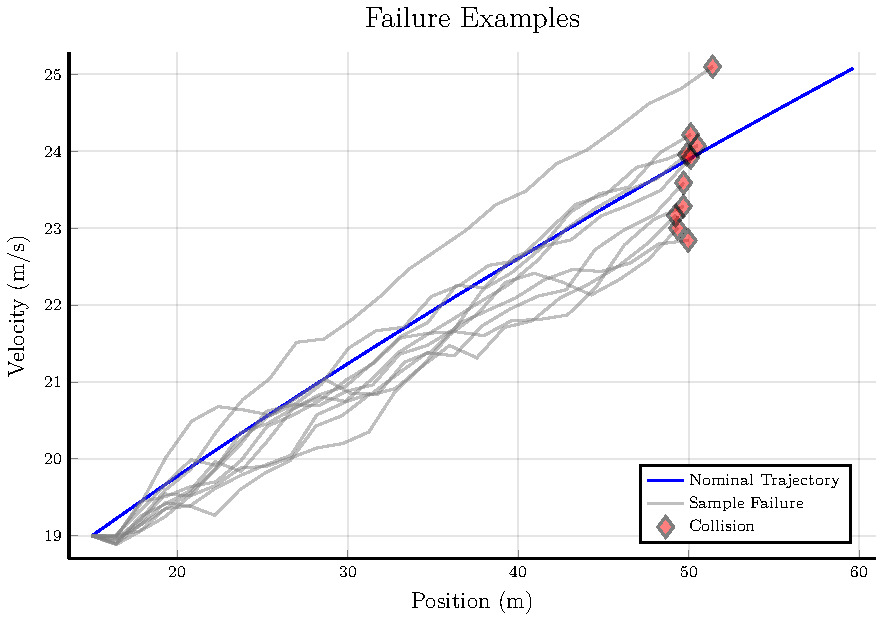
\includegraphics[scale=0.6]{figures/interpretable_validation/2car_sample_failures.pdf}
    \caption{Sample failures that satisfy $\square_{[0, .36]} B \lor d_{\rm maj}$}
    \label{fig:2car_failure_samples}
\end{figure}


\subsection{Pedestrian in Crosswalk}

\paragraph{Scenario 1 - STL on signal}

The disturbances were modeled as zero-mean Gaussian processes with a squared exponential kernel with parameters $\ell = 4$ and $\sigma^2 = 0.5$. The noise was modeled iid as zero mean Gaussians with parameters $\sigma_{r_x} = \sigma_{r_y} = 0.2$ and $\sigma_{v} = 0.5$. The initial condition for the vehicle was ($r_x^{\rm veh}$, $v_x^{\rm veh}$) = (\SI{2.291}{m}, \SI{10.80}{m/s}) and for the pedestrian ($r^{\rm ped}_x$, $r^{\rm ped}_y$, $v^{\rm ped}_x$, $v^{\rm ped}_y$) = (\SI{25}{m}, \SI{-5.93}{m}, \SI{1.78}{m/s}). 


\begin{table}
    \centering
    \caption{Comparison of interpretable validation with STL grammar to baselines for pedestrian scenario.}
    \label{tab:ped_results_stl}
    \begin{tabular}{@{}llll@{}} 
        \toprule
        \textbf{Method} & \textbf{Fail Rate} & \textbf{Log-Likelihood} \\
        \midrule
        Monte Carlo & $0.121 \pm 0.010$ & $4.054 \pm 0.118$  \\
        Cross entropy method (IID) & $0.661 \pm 0.015$ & $\num{-4.564e4} \pm \num{8.001e3}$\\
        Cross entropy method (Trajectory) & $0.990 \pm 0.003$ & $-28.346 \pm 3.174$ \\
        Interpretable validation & $0.883 \pm 0.010$ & $3.553 \pm 0.099$ \\
        \bottomrule
    \end{tabular}
\end{table}

\begin{equation}
\begin{split}
\square_{[1,5]}(&(\delta a_x \leq 1.96) \land (\delta a_y \geq 0.71) \land \\
&(\delta n_x \geq -0.24) \land (\delta n_y \leq 0.53) \land (-0.91 \leq \delta n_v \leq -0.63)) \label{eq:failure_description_pedstl}
\end{split}
\end{equation}

\begin{figure}
    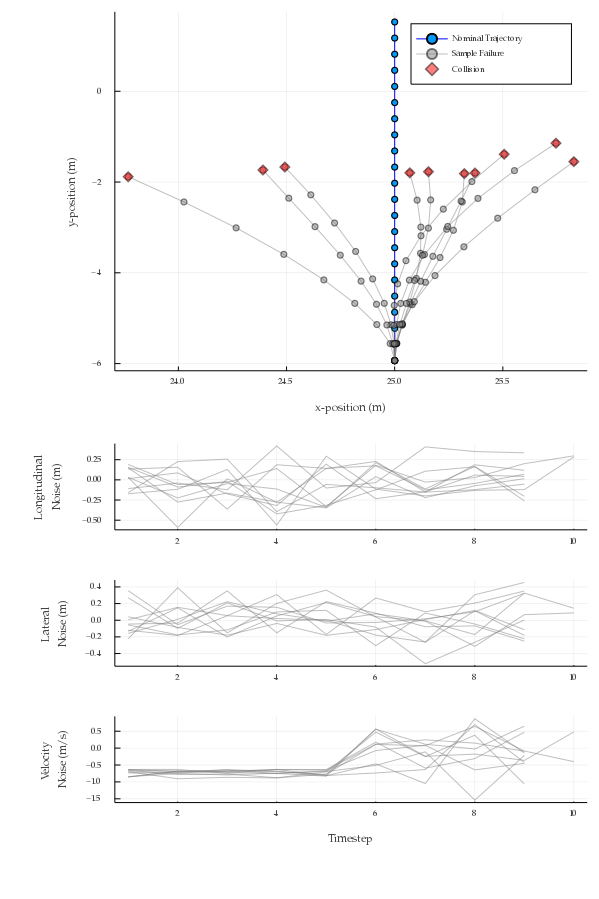
\includegraphics[width=0.85\textwidth]{figures/interpretable_validation/stl_failure_examples.png}
    \caption{Sample failure trajectories from pedestrian STL failure description (\cref{eq:failure_description_pedstl})}
    \label{fig:ped_stl_sample_failures}
\end{figure}


\begin{figure}
    \centering
    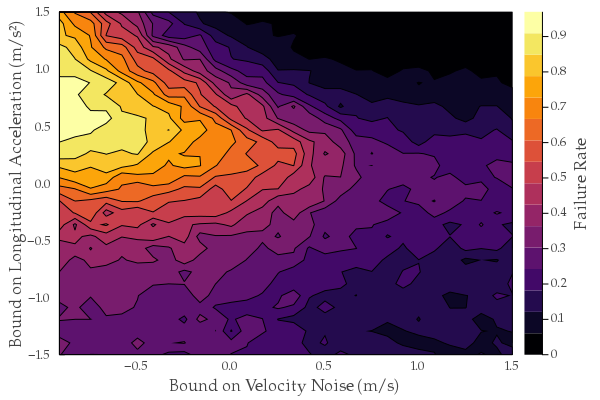
\includegraphics[width=0.8\textwidth]{figures/interpretable_validation/stl_result_sensitivity.png}
    \caption{System sensitivity analysis for longitudinal acceleration bound and velocity noise upper bound}
    \label{fig:stl_ped_sensititivty}
\end{figure}

\paragraph{Scenario 2 - STL on policy}

For the state-dependent setting it is much easier if the disturbances are not correlated over time. We therefore modeled all of the disturbances as zero-mean Gaussians with standard deviations given by $\sigma_{a_x} = \sigma_{a_y} = 1$ and $\sigma_{r_x} = \sigma_{r_y} = \sigma_{v} = 0.5$. The initial condition for the vehicle was ($r_x^{\rm veh}$, $v_x^{\rm veh}$) = (\SI{9.64}{m}, \SI{9.34}{m/s}) and for the pedestrian ($r^{\rm ped}_x$, $r^{\rm ped}_y$, $v^{\rm ped}_x$, $v^{\rm ped}_y$) = (\SI{25}{m}, \SI{-6.99}{m}, \SI{1.94}{m/s}). 

\begin{table}
    \centering
    \caption{Comparison of interpretable validation with state-dependent grammar to baselines for pedestrian scenario.}
    \label{tab:ped_results_state_dependent}
    \begin{tabular}{@{}llll@{}} 
        \toprule
        \textbf{Method} & \textbf{Fail Rate} & \textbf{Log-Likelihood} \\
        \midrule
        Monte Carlo & $0.0 \pm 0.0$ &  -   \\
        Cross entropy method (IID) & $0.184 \pm 0.012$ & $-7.743 \pm 0.264$\\
        Cross entropy method (Trajectory) & $0.566 \pm 0.016$ & $-3.088 \pm 0.003$ \\
        Interpretable validation & $0.997 \pm 0.002$ & $-8.500 \pm 0.166$ \\
        \bottomrule
    \end{tabular}
\end{table}



\begin{equation}
\begin{split}
r_x^{\rm ped} \geq 20.23 &\implies \delta a_y \leq 1.67 \\
r_x^{\rm veh} \geq 16.51 &\implies \delta n_y \geq 1.59 \\
v^{\rm veh} \geq 0.26 &\implies \delta a_y \geq 1.10 \\
(r_x^{\rm veh} \leq 27.87) \lor (r_x^{\rm veh} \geq 15.61) &\implies (\delta n_v \leq 0.20) \land (\delta a_x \leq 1.91)
\end{split} \label{eq:failure_description_ped_state_dep}
\end{equation}

\begin{figure}
    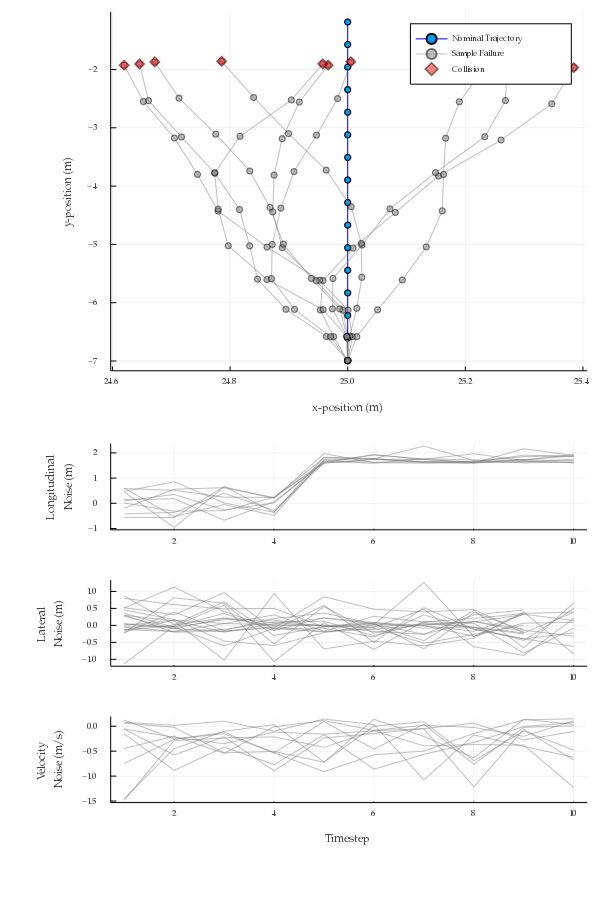
\includegraphics[width=0.85\textwidth]{figures/interpretable_validation/state_dep_failure_examples.png}
    \caption{Sample failure trajectories from pedestrian state-dependent failure description (\cref{eq:failure_description_ped_state_dep})}
    \label{fig:ped_state_dep_sample_failures}
\end{figure}


\begin{figure}
    \centering
    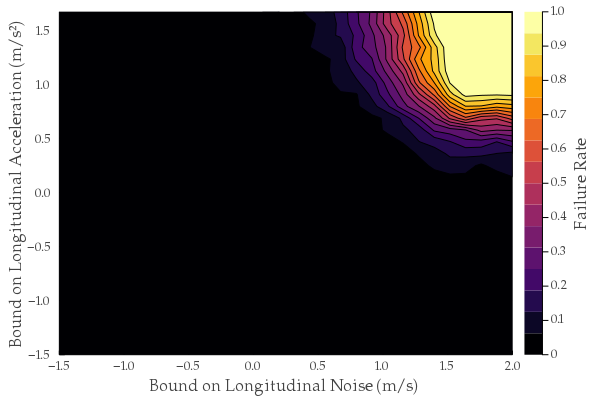
\includegraphics[width=0.8\textwidth]{figures/interpretable_validation/state_dep_result_sensitivity.png}
    \caption{System sensitivity analysis for longitudinal acceleration bound and longitudinal position noise bound}
    \label{fig:ped_state_sensititivty}
\end{figure}



\section{Discussion}

\todo{13 - 1 hr - do a summary of our approach. Describe how it connects to other works, talk about some limitations and future work}
The interpretable failures place minimal constraints on the trajectories so many of the disturbances are selected according to the true model of the environment, leading to the relatively high likelihood of the trajectory. With importance sampling, the distribution causes rare disturbances to be chosen with regularity, even when they are not critical for causing a failure. Many rare events cause the IS trajectories to have very low likelihood.


For an algorithm to be interpretable, its results must be readily understood by a human. Interpretable models must choose an output representation that is sufficiently expressive to compactly convey the desired information while having direct mappings to words and concepts. Decision trees use a branching set of rules to classify data \cite{breiman2017classification} or represent a reinforcement learning policy \cite{rodriguez2019interpretable}. Simple mathematical expressions can be used for regression~\cite{schielzeth2010simple}, governing equation discovery~\cite{brunton2016discovering} and as a reinforcement learning policy~\cite{hein2017particle}. Signal temporal logic (STL) is well-suited for high-dimensional time series data~\cite{lee2018interpretable,vazquez2017logical} because it describes logical relationships between temporal variables and has a natural-language description that is easily understood.